\documentclass{book}
\usepackage[T1]{fontenc}
\usepackage[utf8]{inputenc}
\usepackage[brazil]{babel}
\usepackage{graphicx}
\usepackage{amssymb}
\usepackage{multicol}
\usepackage{hyperref}
\usepackage[a4paper, margin=2cm]{geometry}
\usepackage[framemethod=tikz]{mdframed}
% \usepackage{framed}
\usepackage{titlesec}
\usepackage{enumitem}
\usepackage{xifthen}

\title{Livro de receitas} \author{Karl Jan Clinckspoor} \date{\today}

% Configura o espaçamento dos itens
\setitemize{itemsep=0pt}
\setenumerate{itemsep=0pt}
% Configura o cabeçalho e rodapé
\pagestyle{empty}


% Define se é para colocar figuras e emojis na versão final
\newcommand{\incluirFigura}{true}   
% Cria função para checar se é para colocar figura
\newcommand{\condicionalFigura}[1]{
  \ifthenelse{\equal{\incluirFigura}{true}}%
  {#1}%
  {}
}

% Define como que as receitas são formatadas
\titleformat
    {\section}  % command
    % [display] % shape
    {\Large\bfseries}  % format
    % {Receita \thesection:}  % label
    {}  % label
    {0.5ex}  % sep
    {\centering}  % before-code
    [\vspace{1cm}] % after-code

% Quadros customizados
% Se for para usar figuras, colocar o fundo cinza, senão, sem fundo.
\ifthenelse{\equal{\incluirFigura}{true}}{
  \newmdenv[roundcorner=10pt, backgroundcolor=gray!10,frametitle=Ingredientes,skipabove=0pt]{Ingredientes}
}{
  \newmdenv[roundcorner=10pt, backgroundcolor=white,frametitle=Ingredientes,skipabove=0pt]{Ingredientes}
}
\newmdenv[frametitle=Preparo, skipabove=0pt, linewidth=0]{Preparo}

% Configurar os emojis
\newdimen\emojiheight
\emojiheight=1cm
\newcommand\pimenta{
\includegraphics[height=\emojiheight]{./emojis/pimenta}}
\newcommand{\testado}{
\includegraphics[height=\emojiheight]{./emojis/checkmark}}
\newcommand{\karlAprova}{
\includegraphics[height=\emojiheight]{./emojis/karl_aprova}}
\newcommand{\karenAprova}{
\includegraphics[height=\emojiheight]{./emojis/karen_aprova}}

% Configurar os comandos de receita
% Receita simples, sem os emojis
\newcommand{\receita}[3]{
  \vspace*{0.1cm}
  \section{#1}
  \begin{minipage}[t]{0.3\textwidth} %
    \begin{Ingredientes}
      \noindent
      #2
    \end{Ingredientes}
  \end{minipage}%
  \quad  \begin{minipage}[t]{0.65\textwidth}
    \noindent \begin{Preparo} #3    \end{Preparo}
  \end{minipage}
  \clearpage
}

% Receita com uma caixa adicional de emojis
\newcommand{\receitaemoji}[4][]{
  \vspace*{0.1cm}
  \section{#2}

  % Se é para imprimir figuras, coloca emoji. Senão, não.
  \condicionalFigura{
    % Se tem emoji, coloca na caixa. Senão, fica vazio
    \ifthenelse{%
      \isempty{#1}
    }%
    {}%
    {%
      \begin{mdframed}[userdefinedwidth=4cm, align=center, linewidth=0]
        \centering
        #1
      \end{mdframed}
    }
  }

  \begin{minipage}[t]{0.3\textwidth} %
    \begin{Ingredientes}
      \noindent
      #3
    \end{Ingredientes}
  \end{minipage}%
  \quad  \begin{minipage}[t]{0.65\textwidth}
    \noindent \begin{Preparo} #4    \end{Preparo}
  \end{minipage}
  \clearpage
}

% Entender pq não está funcionando
\newcommand{\receitatrescolsemoji}[6]{
  \vspace*{0.1cm}
  \section{#2}

  % Se for para colocar figura, coloca emoji
  \condicionalFigura{
    % Se tem emoji, colocar, senão, ficar em branco
    \ifthenelse{%
      \isempty{#1}
    }%
    {}%
    {%
      \begin{mdframed}[userdefinedwidth=4cm, align=center, linewidth=0]
        \centering
        #1
      \end{mdframed}
    }
  }

  % Começar os ingredientes
  \begin{minipage}[t]{0.3\textwidth} %
    \begin{Ingredientes}
      \noindent
      #3
    \end{Ingredientes}
  \end{minipage}%
  \quad \begin{minipage}[t]{0.3\textwidth} %
    \begin{Ingredientes}
      \noindent
      #4
    \end{Ingredientes}
  \end{minipage}%
  \quad \begin{minipage}[t]{0.3\textwidth} %
    \begin{Ingredientes}
      \noindent
      #5
    \end{Ingredientes}
  \end{minipage}
  
  \begin{minipage}[t]{\textwidth}
    \noindent \begin{Preparo} #6    \end{Preparo}
  \end{minipage}
  \clearpage
}

% Para receitas com muitos ingredientes, que precisam de cuidados especiais
\newcommand{\receitatrescols}[5]{
  \vspace*{0.1cm}
  \section{#1}
  \begin{minipage}[t]{0.3\textwidth} %
    \begin{Ingredientes}
      \noindent
      #2
    \end{Ingredientes}
  \end{minipage}%
  \quad \begin{minipage}[t]{0.3\textwidth} %
    \begin{Ingredientes}
      \noindent
      #3
    \end{Ingredientes}
  \end{minipage}%
 \quad \begin{minipage}[t]{0.3\textwidth} %
    \begin{Ingredientes}
      \noindent
      #4
    \end{Ingredientes}
  \end{minipage}
  \vfill
  
  \begin{minipage}[t]{\textwidth}
    \noindent \begin{Preparo} #5    \end{Preparo}
  \end{minipage}
  \clearpage
}

% Comando para incluir uma foto de receita sem ter que usar o includegraphics.
% Útil no futuro caso eu queira padronizar alguma coisa
\newcommand{\fotoreceita}[2]{
  \condicionalFigura{
  \begin{center}
    \includegraphics[width=#1]{#2}
  \end{center}
  }
}

% Comando para facilitar colocar temperaturas
\newcommand{\grau}{$^\circ$}

% Início do documento
\begin{document}

% Seleciona a fonte
% \fontfamily{phv}\selectfont
% \maketitle
% \tableofcontents

% \chapter{Receitas salgadas}
% \condicionalFigura{
% 	\begin{center}
% 		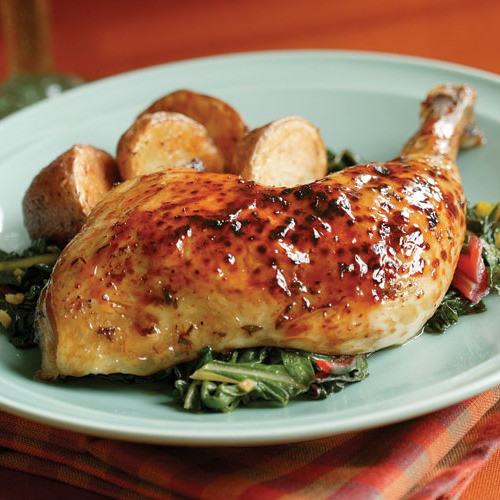
\includegraphics[width=0.7\textwidth]{./Fotos/foto_savory}\end{center}
% }
% \clearpage
% \receita{Stir Fry de Frango\checkmark}{
	\begin{itemize}
		\item 1 meio-peito de frango
		\item Verduras apropriadas (cenoura, brócolis, acelga)
		\item 1 dente de alho
		\item Molho shoyu
		\item Óleo para fritar
		\item Gengibre, bem pouco.
	\end{itemize} }{
	\begin{enumerate}
		\item Cortar o frango em tirinhas
		\item Ralar 1 dente de alho inteiro.
		\item Colocar um pouco de óleo numa frigideira ou wok, e colocar o alho ralado
		      e gengibre por alguns segundos.
		\item Colocar o frango quando a panela já estiver quente. Virar bastante para
		      não deixar queimar.
		      \begin{itemize}
			      \item Se não estiver quente o suficiente, o frango irá perder água e vai
			            ficar seco.
			      \item Se tiver muito frango, fazer a fritura do mesmo em várias porções, de
			            acordo com o tamanho da frigideira e da potência do fogo.
		      \end{itemize}
		\item Quando dourado, retirar o frango e colocar armazenado em outro lugar.
		\item Fritar as verduras e legumes até ficarem cozidas.
		      \begin{itemize}
			      \item Colocar sempre os mais duros antes
			      \item Caso tenha brócolis, branquear (ferver água, deixar 2-3 minutos,
			            escorrer)
			      \item Caso tenha acelga, coloque por último
		      \end{itemize}
		\item Voltar o frango, aquecer um pouco, colocar 1 colher de sopa de shoyu,
		      mexer bem para incorporar. Vai ficar mais escuro do que aparenta no
		      início. \begin{itemize} \item Se tiver macarrão, colocar o shoyu antes,
			            incorporar, depois colocar o macarrão. \item Tomar cuidado com não deixar
			            a tampa do shoyu sair e derramar demais. \end{itemize}
	\end{enumerate}

	\fotoreceita{0.7\textwidth}{./Fotos/Stir_Fry.png} }

\receita{Bife com Curry\checkmark}{
	\begin{itemize}
		\item Carne
		\item Alho
		\item Cebola
		\item Óleo/manteiga
		\item Curry em pó
	\end{itemize} }{
	\begin{enumerate}
		\item Cortar a carne em tiras
		\item Fritar cebola e alho bem picadinho, refogar com óleo ou manteiga,
		      colocar a carne e refogar uns minutos.
		      \begin{enumerate}
			      \item Como vai usar curry, pode soltar água da carne.
			      \item Caso não solte a água, abaixa o fogo e coloca a tampa e espera um
			            pouco. Caso não solte ainda, coloca meio copo de água quente.
		      \end{enumerate}

		\item Aí põe algo como uma colher de sopa de curry e termina de refogar. Serve
		      com arroz.
	\end{enumerate} }

\receita{Arroz padrão na panela de arroz\checkmark}{
	\begin{itemize}
		\item Arroz normal. Geralmente, para 2, um copo é o suficiente.
		\item Alho. Para 2, meio alho está bom.
		\item Cebola. Para 2, meia cebola pequena está bom
		\item Óleo. Suficiente para cobrir o fundo da panela com um filmezinho.
		\item Água quente
	\end{itemize}
}
{
	\begin{enumerate}
		\item (Opcional) Colocar a água para esquentar. Se fizer isso, diminui o
		      tempo de cozimento.
		\item Colocar o alho e cebola finamente picados numa panela com óleo para
		      dourar.
		      \begin{itemize}
			      \item Pode adicionar o alho depois para diminuir a
			            chance de queimar ele.
		      \end{itemize}
		\item Colocar o arroz e fritar um pouquinho. Transferir tudo para a panela de
		      arroz. Colocar a água na proporção de 2 copos de água para 1 copo de arroz
		      (medida da panela).
		\item O tempo médio de cozimento registrado aqui é de aproximadamente 13-15
		      minutos.
		\item O fundo da panela sempre fica grudado. Tentar achar uma maneira de
		      fazer isso parar de acontecer.
	\end{enumerate}
}

\receita{Arroz arbório na panela de arroz\checkmark}{\label{rec:arroz_arborio_panela}
	\begin{itemize}
		\item Arroz arbório, ou algum tipo de arroz para risoto
		\item Água, na proporção aproximada de 2x o ``volume'' de arroz.
	\end{itemize}
}{
	\begin{enumerate}
		\item Colocar o arroz arbório na panela e colocar a água. Deixar cozinhar.
		\item O resultado é um arroz que parece arroz japonês. Fica bem fofinho,
		      expandido, e contrasta bem com pratos mais fortes, como frango tailandês ou
		      outros \emph{stir-frys}.
	\end{enumerate}
}

\receita{Pique Macho\checkmark}{
	\begin{itemize}
		\item Batata para fritar
		\item Cebola roxa
		\item Tomate
		\item Pimentão (locoto)
		\item Salsicha
		\item Lombo
		\item Pimenta do reino
		\item Cominho
		\item Mostarda
		\item Shoyu (relativamente pouco, 2 colheres para 1kg de carne)
		\item Sal
		\item Óleo de girassol
		\item Ovos
		\item Maionese
		\item Ketchup
	\end{itemize} }{
	\begin{enumerate}
		\item Fritar as batatas
		\item Fritar a carne, sem se preocupar em selar. Parte do sabor do prato vem
		      do líquido soltado pela carne.
		\item Colocar o cominho, pimenta, mostarda, shoyu e sal com a carne ainda
		      vermelha.
		\item Colocar os ovos para cozinhar em outra panela.
		\item Deixar a carne cozinhar.
		\item Colocar a salsicha e esperar 5 minutos, desligar o fogo.
		\item Colocar a carne sobre as batatas fritas.
		\item Colocar as cebolas que estavam no vinagre para perder o sabor forte,
		      tomate, ovos cozidos, pimentões verdes, sobre o prato.
	\end{enumerate}

	\fotoreceita{0.7\textwidth}{./Fotos/pique_macho}

}

\receita{Macarrão com manteiga, ovo e queijo\checkmark}{
	\begin{itemize}
		\item Espaguete (80 g para uma pessoa)
		\item Sal
		\item 3/4 copo de leite
		\item 1 ovo
		\item 2 colheres de manteiga
		\item 2/3 copo de parmesão ralado
		\item Pimenta a gosto
	\end{itemize} }{
	\begin{enumerate}
		\item Cozinhar o macarrão numa panela. \begin{itemize}
			      \item Colocar sal na água. Deixar ferver. Colocar macarrão.
		      \end{itemize}
		\item Escorrer o macarrão ao ficar al dente.
		\item Devolver o macarrão na panela, abaixar a temperatura, colocar a mistura
		      de leite, ovo e manteiga, e mexer até recobrir o macarrão. \begin{itemize}
			      \item Quando eu fiz, deixei bastante tempo para garantir que o ovo estivesse
			            cozido. Ele engrumou, mas a Karen gostou de qualquer forma.
		      \end{itemize}
		\item Remover o calor. Colocar queijo e misturar. Se estiver pastoso demais,
		      colocar mais lente.
	\end{enumerate} }

\receita{Caldo de frango\checkmark\label{rec:caldo_frango}}{
	\begin{itemize}
		\item 3 dentes de alho
		\item 1 cebola pequena
		\item 2 coxas de frango, 2 sobrecoxas de frango, 2 meio-peitos
		\item Óleo
		\item Sal
	\end{itemize} }{
	\begin{enumerate}
		\item Cortar bem pequeno o alho e a cebola. Colocar ambos para dourar um pouco
		      de tempo. Colocar uma colher de chá de sal.
		\item Colocar o frango, sem tirar a pele ou qualquer outra coisa.
		\item Colocar a água. Cerca de 2 litros, ou até cobrir tudo. Deixar a panela
		      no fogo alto até a água começar a ferver, depois colocar no fogo médio.
		\item Tempo total é de cerca de 1h depois de começar a ferver. Mexer no frango
		      de vez em quando para ver a textura e possivelmente abrir os pedaços para
		      ajudar a cozinhar.
		      \begin{itemize}
			      \item Dá para remover o peito antes dos outros porque deve cozinhar antes, e
			            se ficar tempo demais fica duro.
		      \end{itemize}
		\item Estará pronto quando notar que a carne está saindo dos ossos.
		\item Coar tudo por uma peneira. Reservar o frango para fazer uma torta ou
		      alguma coisa assim.
	\end{enumerate} }

\receita{Risoto de parmesão\checkmark}{
	\begin{itemize}
		\item 2,5 copos de caldo de frango (vide receita \ref{rec:caldo_frango})
		\item 0,75 copos de água
		\item 2 colheres de sopa de manteiga
		\item 0,5 cebola grande, finamente cortada
		\item Sal, pimenta
		\item 0,5 dente de alho, cortado finamente
		\item 1 copo de arroz para risoto (arbório ou outro)
		\item 25-30g de parmesão ralado
		\item 1 colher de sopa de salsinha e cebolinha
		\item 0,5 colher de sopa de suco de limão
	\end{itemize} }{
	\begin{enumerate}
		\item Ferver o caldo e a água em panela grande em fogo quente. Depois reduzir
		      o calor para um fervor gentil.
		\item Derreter metade da manteiga numa panela\footnote{De preferência de
			      ferro, mas pode ser alguma com uma massa térmica maior que uma panela
			      comum} em calor médio. Colocar a cebola e 0,75 colher de sopa de sal. Ir
		      mexendo por 5 a 7 minutos.
		\item Colocar o alho até ficar cheiroso, 30 segundos.
		\item Colocar o arroz e cozinhar, mexendo lentamente até os grãos ficarem
		      translúcidos nas bordas, 3 minutos.
		      \begin{itemize}
			      \item Cuidado com deixar o arroz queimar nesta etapa! Mexer bastante.
		      \end{itemize}
		\item Colocar o caldo aquecido até cobrir o arroz. Reduzir o calor para
		      médio-baixo. Ficar mexendo até absorver. Quando secar, adicionar mais caldo
		      em parcelas bem pequenas. Sempre ficar mexendo para garantir que não vai
		      queimar. Continuar até o arroz ficar cremoso e cozido, ou acabar o caldo.
		      16-19 minutos.
		\item Colocar o parmesão e mexer. Remover do calor, cobrir, e deixar parado
		      por 5 minutos.
		\item Colocar o resto da manteiga, salsinha, cebolinha e limão.
		      \begin{itemize}
			      \item O limão não foi muito bem quisto pela Karen. Dá para colocar a
			            salsinha e cebolinha, separar em duas metades, e em uma delas colocar 0,25
			            colher de sopa do suco de limão.
		      \end{itemize}
	\end{enumerate}

	\fotoreceita{0.7\textwidth}{./Fotos/Risoto.png} }

\receita{Conchiglioni de queijo\checkmark}{
	\begin{itemize}
		\item Aproximadamente 50 Conchiglioni
		\item 1 cilindro de ricota fresca. Mais molinha é melhor (cerca de 200g?)
		\item 1 pote de creme de ricota.
		\item 100g de mussarella ralada
		\item 100g de provolone ralado
		\item 25g de parmesão ralado para recheio, um pouco para polvilhar em cima
		\item molho de tomate pronto. 1 saquinho para pouco molho, 2 para banhar bem.
		\item sal
		\item nozes picadas, aproximadamente 8
	\end{itemize} }{
	\begin{enumerate}
		\item Cozinhar os conchiglioni em água com sal até ficarem no ponto.
		\item Enquanto cozinha, misturar todos os queijos juntos, com as nozes. Provar
		      se tem sal suficiente e colocar um queijo ou outro para atingir o sabor.
		      Senão, colocar sal, mas por experiência, para meu gosto, isso não é
		      necessário.
		\item Ao terminar, coar o macarrão, deixar esfriar um pouco. Começar a aquecer
		      o forno a 200 $^\circ$C.
		\item Numa travessa grande, cobrir a base com molho de tomate, para evitar do
		      macarrão queimar durante o assamento.
		\item Preencher generosamente os conchiglioni com o recheio. Colocar na
		      travessa da maneira mais eficiente possível, porque 50 conchiglioni é
		      bastante.
		\item Jogar molho por cima deles, tentando ser homogêneo, mas não é
		      necessário. Após, salpicar parmesão a gosto.
		\item Colocar no forno por 15 minutos. Se tiver duas travessas, retirar a
		      travessa de baixo, mais perto do fogo, antes, para que não queime. O
		      interessante é derreter o recheio e aquecer tudo, pois a comida já está
		      tecnicamente pronta para ser comida.
		\item Servir e comer imediatamente. O que sobrar pode ser resfriado ou
		      congelado e posteriormente aquecido no micro ondas que não há perda de
		      sabor.
	\end{enumerate}

	\fotoreceita{0.5\textwidth}{./Fotos/conchiglioni} }

\receita{Frango tailandês com manjericão\checkmark}{
	\begin{itemize}
		\item 1 meio peito de frango
		\item 1 a 2 pimentas vermelhas, a critério pessoal
		\item 2 a 4 dentes de alho
		\item 1 a 2 colheres de sopa de shoyu
		\item 1 colher de chá de açúcar cristal.
		\item 1 ramo de manjericão
		\item 1 colher de sopa de molho de ostra (opcional)
	\end{itemize} }{
	\begin{enumerate}
		\item Se for fazer arroz, já colocar para cozinhar agora que vai acabar
		      terminando aproximadamente junto com o frango. Vide receita
		      \ref{rec:arroz_arborio_panela}.
		\item Cortar o frango em pedaços \emph{bite-sized} e reservar. Quanto for
		      menor o pedaço de frango, mais rápido ele ficará cozido e menor será a
		      chance de queimar os temperos. Fatias do tamanho de um dedo fino pareceram
		      apropriadas.
		\item Macerar a pimenta e o alho juntos
		      \begin{itemize}
			      \item Se utilizar alho já picado, só precisa misturar.
		      \end{itemize}
		\item Separar as folhas do manjericão do caule e lavar.
		\item Misturar o shoyu, molho de ostra e açúcar cristal numa xícara.
		\item Começar a aquecer o wok com óleo até ficar bem quente
		\item Fritar o macerado de alho e pimenta por alguns segundos, mexendo sempre
		      \begin{itemize}
			      \item Se utilizar alho já picado, cuidado que espirra bastante! Adicionar
			            com o óleo menos quente.
		      \end{itemize}
		\item Acrescentar o frango e \emph{stir fry} por 2 minutos. Não pode estar cru nem
		      cozido demais
		      \begin{itemize}
			      \item Se achar que está pouco cozido porque os pedaços estão
			            grandes, deixar cozinhar por um pouco mais. Abaixar o fogo se
			            começar a queimar a pimenta e o alho.
		      \end{itemize}
		\item Acrescentar o molho de soja, de ostra, açúcar e mais \emph{stir fry} por 15
		      segundos.
		\item Acrescentar o manjericão, misturar, e desligar o fogo imediatamente.
		\item Servir bem quente com arroz pré-preparado e guarnecer com ovo por cima
		      \begin{enumerate}
			      \item Não achei necessário temperar o ovo, pois o prato em si já possui
			            bastante sabor.
		      \end{enumerate}

	\end{enumerate}

	\fotoreceita{0.5\textwidth}{./Fotos/frango_tailandes}
}

\receita{Panqueca salgada}{
	\begin{itemize}
		\item 3 ovos
		\item 200 mL de leite integral
		\item 100 g de farinha de trigo
		\item 50 g de manteiga derretida
		\item sal
	\end{itemize} }{
	\begin{itemize}
		\item Peneirar a farinha.
		\item Fazer um buraco no meio da farinha e colocar os ovos. Mexer com fouet.
		\item Colocar o leite aos poucos para não formar pelotas.
		\item Derreter a manteiga numa panela separada e incorporar na massa.
		\item Descansar a massa por pelo menos 1h, idealmente 5, na geladeira.
		\item Untar uma frigideira e fritar em camadas bem finas, em fogo médio/alto.
	\end{itemize} }

\receita{Ovos diabólicos}{
	\begin{itemize}
		\item Ovos
		\item Creamcheese
		\item Pimenta vermelha
		\item Sal
		\item Mostarda
	\end{itemize} }{
	\begin{enumerate}
		\item Cozinhar os ovos por 5 minutos, colocando-os em água gelada
		      posteriormente para ajudar a soltar a casca.
		\item Cotar os ovos perpendicularmente para tirar as gemas.
		\item Misturar as gemas com creamcheese, pimenta vermelha, sal, mostarda.
		\item Quando a mistura estiver bem lisa, sem grumos, colocar num saquinho,
		      cortar a ponta e preencher os espaços da gema na clara cozida.
	\end{enumerate} }

\receita{Nhoque a bolonhesa\checkmark}{

	\textsc{Nhoque}

	\begin{itemize}
		\item 600g de batatas Asterix
		\item 1 ovo
		\item 2 xícaras de chá de parmesão ralado fino
		\item 1 colher de sopa de manteiga
		\item Pimenta síria a gosto
		\item 1 colher de sopa de farinha de trigo
		\item 1 fio de azeite e sal para a água do cozimento
	\end{itemize}

	\textsc{Molho bolonhesa\checkmark} \label{rec:molho_bolonhesa}

	\begin{itemize}
		\item 1 colher de sopa de óleo ou azeite
		\item 1 cebola média picada
		\item 2 dentes de alho
		\item 1 kg de carne moída
		\item Orégano
		\item Pimenta do reino
		\item Colorau
		\item Sal
		\item 1 lata de extrato de tomate
		\item 1 sachê de molho de tomate
		\item 1 xícara de chá de água
	\end{itemize} }{

	\textsc{Nhoque}

	\begin{enumerate}
		\item Cozinhar as batatas, amassar ainda quente. (com casca?)
		\item Aguardar as batatas esfriarem. Adicionar os outros ingredientes até
		      formar uma massa tipo pão leve. Se necessário, adicionar mais farinha (o que
		      observar?)
		\item Ferver água com um fio de azeite.
		\item Fazer rolinhos e cortar a massa em tubos curtos. Colocar na água
		      fervente.
		\item Quando a massa boiar, retirar da água.
	\end{enumerate}

	\textsc{Molho bolonhesa}
	\begin{enumerate}
		\item Numa panela média, refogue a cebola e o alho no óleo ou no azeite até
		      dourar.
		\item Em seguida adicione a carne moída e tempere com orégano, pimenta do
		      reino, colorau, sal a gosto.
		\item Mexer para misturar bem e refogar por aproximadamente 10 minutos.
		\item Adicionar o extrato, molho e água.
		\item Misturar, tampar a panela e deixar cozinhar por mais 5 minutos.
		\item Desligar o fogo
	\end{enumerate}

	\fotoreceita{0.7\textwidth}{./Fotos/Nhoque} }

\receita{Vinagretes}{
	\begin{multicols}{2}

		\textsc{clássico}
		\begin{itemize}
			\item 1 pitada de sal
			\item 1 pitada de pimenta (do reino ou branca)
			\item 1 colher de sopa de vinagre
			\item 3 colheres de sopa de óleo vegetal
		\end{itemize}

		\textsc{mostarda}
		\begin{itemize}
			\item 1 pitada de sal
			\item 1 pitada de pimenta (do reino ou branca)
			\item 1 colher de chá de mostarda (Dijon)
			\item 1 colher de sopa de vinagre
			\item 3 colheres de sopa de óleo vegetal
		\end{itemize}

		\textsc{azeite}
		\begin{itemize}
			\item 1 pitada de sal
			\item 1 pitada de pimenta (do reino ou branca)
			\item 1 colher de sopa de vinagre
			\item 1 colher de sopa de suco de limão
			\item 4 colheres de sopa de azeite
		\end{itemize}

		\textsc{balsâmico}
		\begin{itemize}
			\item 1 pitada de sal
			\item 1 pitada de pimenta (do reino ou branca)
			\item 1 colher de sopa de vinagre balsâmico
			\item 1 colher de sopa de suco de limão
			\item 3 colheres de sopa de azeite
			\item meio dente de alho finamente picado
		\end{itemize}

		\textsc{chalota\footnote{Chalota é basicamente um tipo de cebola}}
		\begin{itemize}
			\item 1 pitada de sal
			\item 1 pitada de pimenta (do reino ou branca)
			\item 1 colher de sopa de vinagre
			\item 3 colheres de sopa de óleo vegetal
			\item 1 pequena chalota cortada finamente (direção do comprimento)
		\end{itemize}

		\textsc{mostarda e mel}
		\begin{itemize}
			\item 1 pitada de sal
			\item 1 pitada de pimenta (do reino ou branca)
			\item 1 colher de chá de mostarda Dijon
			\item 1 colher de chá de mel (fluído)
			\item 1 colher de sopa de vinagre de mel
			\item 3 colheres de sopa de azeite ou óleo vegetal
			\item 1 colher de chá de chalota cortada
		\end{itemize}

	\end{multicols} } {
	\begin{enumerate}
		\item Colocar sal e pimenta numa tigela
		\item Adicionar 1 colher de sopa de vinagre até dissolver o sal
		\item Adicionar 3 colheres de sopa de óleo, e misturar até incorporar bem o
		      vinagre e o óleo.
		\item Adicionar as ervas e outros flavorizantes.
	\end{enumerate} }

\receita{Moussaka\checkmark}{

	\textsc{Moussaka}
	\begin{itemize}
		\item 6 batatas médias
		\item 500g de carne moída
		\item 5 tomates ou molho de tomate pronto
		\item 1 cebola
		\item azeite
		\item 30 g de manteiga
		\item uma colher de chá de canela
		\item uma colher de sopa de mel
		\item noz-moscada
		\item sal, pimenta
	\end{itemize}

	\textsc{Bechamel}
	\begin{itemize}
		\item 20 g de manteiga
		\item 3 colheres de sopa rasas de farinha
		\item 350 mL de leite
	\end{itemize}
}{
	\begin{enumerate}
		\item Cortar as cebolas e refogar em panela pequena. Colocar os tomates ou
		      molho de tomate. Colocar o azeite, canela, mel, sal, pimenta. Caso seja
		      feito com tomate, reduzir por 25 minutos em fogo médio. Senão, reduza
		      somente o quanto achar necessário.
		\item Descascar e cortar as batatas em fatias finas.
		\item Dispor as batatas no fundo de uma travessa untada com manteiga alta o
		      suficiente para caber todos os ingredientes. Colocar um pouco do molho de
		      tomate nas batatas.
		\item Levar ao forno bem forte (grelha) por 8 a 12 minutos para dourar as
		      batatas.
		\item Cozinhar a carne moída na manteiga em fogo forte com sal e pimenta.
		      Cozinhar até soltar toda a água.
		\item Adicionar o molho de tomate e reduzir, em fogo baixo.
		\item Remover a batata do forno, regular a temperatura para 200\grau C.
		\item Para fazer o bechamel, em uma panela pequena, jogar 20 g de manteiga,
		      adicionar a farinha até obter uma mistura homogênea. Incorporar o leite
		      devagar, sem parar de mexer. Juntar sal, pimenta e noz moscada.
		\item Por cima da batata, colocar uma camada de carne, outra camada de batata,
		      até acabar com tudo ou encher a travessa. Cobrir com o molho bechamel.
		\item Assar a 200 \grau C por 50 minutos a uma hora. Idealmente o bechamel irá
		      ficar dourado.
	\end{enumerate}


	\fotoreceita{0.45\textwidth}{./Fotos/Moussaka.jpg} \fotoreceita{0.45\textwidth}{./Fotos/Moussaka2.jpg}
}

\receita{Lentilha com Curry\checkmark}{
	\begin{itemize}
		\item 100 g de lentilha vermelha (ideal) ou verde
		\item meia cebola média picada
		\item 1 dente de alho
		\item 1/2 cubos de Golden Curry (já contém sal) ou 1 colher e meia de Curry
		      Kitano com meia colher rasa de sopa de sal. Alternativamente:
		      \begin{itemize}
			      \item 1 colher de café de pimenta chili
			      \item 1 colher de café de cominho
			      \item 1 colher de café de coentro em sementes esmagadas
			      \item 1 colher de café de sal
		      \end{itemize}
		\item meio litro de água quente
	\end{itemize}
}{
	\begin{enumerate}
		\item Lavar a lentilha e cozinhar na água por uns 20 minutos. Checar de 5 em
		      5 minutos depois de 10 minutos de cozimento. Se for vermelha, é mais rápida.
		\item Refogar a cebola e o alho até amolecer um pouco, não precisa dourar.
		\item Se não tiver o Golden curry, acrescentar os temperos à cebola para despertar o
		      sabor e não deixar queimar. Refogar por 5 segundos.
		\item Jogar a lentilha cozida com água na cebola refogada. Misturar bem. Se
		      for usar o Golden Curry, colocar 1 tablete e esperar dissolver. Provar. Se
		      precisar de mais, colocar ou sal ou mais curry.
	\end{enumerate}

	\fotoreceita{0.3\textwidth}{./Fotos/LentilhaComCurry}
}

\receita{Vagem refogada\checkmark}{
	\begin{itemize}
		\item 1 pacotinho de vagem de mercado (chuto 20 vagens)
		\item 1/3 de cebola média
		\item Meio dente de alho ou quantidade equivalente de pasta de alho
		\item Sal a gosto
	\end{itemize}
}{
	\begin{enumerate}
		\item Cortar a cebola em pedaços relativamente pequenos, cubinhos.
		\item Lavar a vagem, tirar a ponta e o fiozinho. Esse fio vai da ponta até o
		      outro lado, passando pelo lado externo. Tirar a ponta com os dedos pode
		      ajudar a remover essa parte, mas não é necessário.
		\item Colocar a cebola na frigideira com óleo, já quente, sob temperatura
		      média, e refogar por aproximadamente 5 minutos, ou até começar a dourar um
		      pouco.
		\item Colocar o alho e fritar por poucos segundos, só até deixar o aroma sair.
		      Colocar o sal.
		\item Colocar a vagem, mexer bem no começo, depois deixar tostar um pouco.
		      Virar de vez em quando para garantir cozimento por completo. Provar depois
		      de cerca de 10 minutos e ir provando depois até ficar bom.
		\item Servir imediatamente.
	\end{enumerate}
}
\receita{Macarrão de abobrinha\checkmark}{
	\begin{itemize}
		\item 1 abobrinha grande
		\item Molho bolonhesa (vide \ref{rec:molho_bolonhesa})
		\item (opcional) Espaguete
		\item Cebola
		\item Alho
	\end{itemize}
}{
	\begin{enumerate}
		\item Lavar a abobrinha, passar ela no equipamento para fazer os fios
		\item Refogar a cebola até quase dourar, colocar o alho e o sal, e colocar a
		      abobrinha. Mexer um pouco.
		\item Fechar com uma tampa e deixar assim por 5 minutos.
		\item Se desejado, misturar com espaguete e servir imediatamente com o molho.
	\end{enumerate}
}

\receita{Tapioca de ovo\checkmark}{
	\begin{itemize}
		\item Farinha de tapioca
		\item Ovo
	\end{itemize}
}{
	\begin{enumerate}
		\item Não há muito truque para esta receita. Colocar um tanto de tapioca e um
		      tanto de ovo. Misturar. A consistência deve ficar similar à uma panqueca.
		\item Colocar no fogo, deixar tomar forma, depois colocar algum recheio, como
		      queijo. Servir quente.
	\end{enumerate}
}

\receita{Bife acebolado\checkmark}{
	\begin{itemize}
		\item 2 bifes de contra-filé
		\item 1/4 de cebola média
		\item Sal a gosto
	\end{itemize}
}{
	\begin{enumerate}
		\item Colocar o bife na frigideira com um fio de óleo vegetal
		\item Colocar a cebola logo em seguida. Remover quando a carne estiver pronta.
		      \begin{itemize}
			      \item Caso a cebola ainda não esteja boa, mas a carne sim, deixar a
			            cebola sozinha por um pouco mais de tempo.
		      \end{itemize}
	\end{enumerate}
}


\receita{Batata frita no airfryer\checkmark}{
	\begin{itemize}
		\item Batata congelada
		\item Sal a gosto
	\end{itemize}
}{
	\begin{enumerate}
		\item Colocar a batata congelada no airfryer, nas condições mostradas no
		      equipamento.
		      \begin{itemize}
			      \item  Se não tiver uma pequena quantidade de óleo na superfície da
			            batata, envolvê-la com um pouco.
		      \end{itemize}
		\item Remover, colocar num prato, e colocar sal a gosto.
	\end{enumerate}
}

\receita{Quiche}{

	\textsc{Massa para quiche salgada}

	\begin{itemize}
		\item 200 g de farinha
		\item 100 g de manteiga sem sal gelada
		\item 1 ovo batido
		\item 2 ou 3 colheres de água gelada
		\item sal
	\end{itemize}

	\textsc{Recheio 1: Queijo branco, parmesão e alho poró}

	\begin{itemize}
		\item 150 g de queijo minas frescal em cubos pequenos
		\item 50 g de parmesão ralado
		\item 50 mL de leite
		\item 50 mL de creme de leite 35\% (não usar de caixinha, pois talha em altas
		      temperaturas)
		\item 2 ovos batidos
		\item orégano
		\item 1 xícara de alho poró em fatias
	\end{itemize}

	\textsc{Recheio 2: Muçarela e tomate seco}

	\begin{itemize}
		\item 150 g de muçarela ralada
		\item 2 ovos batidos
		\item 50 mL de leite
		\item 50 mL de creme de leite 35\%
		\item noz moscada
		\item manjericão fresco picado
		\item 4 metades de tomate seco
	\end{itemize}

	\textsc{Recheio 3: Quiche Lorraine}

	\begin{itemize}
		\item 250 g de bacon em tiras, fritos e secos em papel toalha
		\item 3 ovos
		\item 250 mL de creme de leite 35\%
		\item 100 g de queijo gruyere ralado
	\end{itemize}

	\textsc{Recheio 4: Batata e bacon}

	\begin{itemize}
		\item 1 batata cortada em fatias finas
		\item 100 g de bacon em tiras, fritos e secos em papel toalha
		\item 2 ovos
		\item 120 mL de creme de leite 35\%
		\item 100 mL de leite
		\item 1 colher de chá de salsinha fresca picada
		\item 50 g de queijo emmental ralado
	\end{itemize}
}{

	\textsc{Preparo da massa, pré-assamento}

	\begin{enumerate}
		\item Pré-aquecer o forno a 200\grau{} C.
		\item Peneirar a farinha e o sal. Colocar no processador.
		\item Acrescentar a manteiga em cubos ao processador no modo pulse até formar
		      uma consistência de farofa.
		\item Acrescentar o ovo batido e depois a água até formar uma bola. Não
		      manipular muito, envolver em filme plástico e guardar na geladeira por 1
		      hora.
		\item Após 1 hora, abrir com rolo sobre papel manteiga.
		\item Virar a massa para a forma com o auxílio do papel, moldar ajustando as
		      bordas e preenchendo as falhas com pedacinhos de massa.
		      \begin{itemize}
			      \item Se assar assim, a massa vai descer e o fundo vai subir, então é
			            necessário assar com peso.
		      \end{itemize}
		\item Colocar feijões sobre papel manteiga, sobre a massa, cobrindo todo o
		      fundo e uns 2 ou 3 cm de altura.
		\item Assar por 10 minutos com os feijões, depois retirá-los, e depois assar
		      por mais 10 minutos.
		\item O recheio só pode ser colocado com a massa pré-assada.
	\end{enumerate}

	\textsc{Assamento dos recheios}

	\begin{itemize}
		\item[Recheio 1] Distribuir na massa assada os queijos, o alho poró e o
		      orégano. Cobrir com a mistura de ovos, leite e creme de leite e assar por
		      35/45 minutos a 180\grau{} C.
		\item[Recheio 2] Distribuir na massa assada o queijo, tomate seco e
		      manjericão. Bater os ovos, leite e creme, temperar com um pouco de sal e noz
		      moscada e cobrir. Assar por 35/45 minutos a 180\grau{} C.
		\item[Recheio 3] Bater os ovos e o creme e temperar com pimenta e noz moscada.
		      Espalhar o queijo e o bacon na massa e cobrir com a mistura de ovos. Assar
		      por 35/45 minutos a 180\grau{} C.
		\item[Recheio 4] Bater os ovos, leite e o creme e temperar com salsinha.
		      Espalhar o bacon e o queijo na massa e cobrir com a mitura de ovos. Assar
		      por 35/45 minutos a 180\grau{} C.
	\end{itemize}
}

\receita{Kebab de frigideira\checkmark}{
	\begin{itemize}
		\item 300 g de carne moída (usei ponta de alcatra)
		\item 1 copo de arroz
		\item 1 cebola pequena (ou meia cebola média)
		\item Sal
		\item Pimenta do reino
		\item Pimenta síria
		\item 4 colheres de chá de óleo vegetal
	\end{itemize}
}{
	\begin{enumerate}
		\item Misturar a cebola ralada com a carne moída numa travessa grande
		\item Adicionar sal (5 giradas), pimenta do reino (2 pitadas), pimenta
		      síria (generosamente, 1 colher de sopa cheia), e misturar bem
		\item Colocar o óleo na frigideira e cobrir bem
		\item Espalhar a carne e abrir na frigideira. Tentar formar uma boa
		      estrutura, não deixar buracos
		\item Colocar o arroz na panela de arroz com 2 copos de água
		\item Colocar a frigideira no fogo médio
		\item Em aproximadamente 3 minutos a água irá começar a sair
		\item Após cerca de 5-8 minutos, corte em tiras de 1-2 polegadas, com um pão
		      duro ou uma espátula
		\item Quando achar que um dos lados está dourado o suficiente, virar.
		\item Quando o outro lado terminar de cozinhar, servir imediatamente.
		      \begin{itemize}
			      \item Aqui, demorou cerca de 20 minutos tudo, e as tiras principais de
			            carne não ficaram tão douradas quanto gostaria, mas os pedaços avulsos
			            estavam bem saborosos. A cebola irá dourar também e dar um bom sabor
		      \end{itemize}
	\end{enumerate}
}
% Receitas que a Karen tem que me passar:
% Receita de omelete de forno com vegetais, que fez no dia 26/01/2020

%%% Local Variables:
%%% mode: latex
%%% TeX-master: "main"
%%% End:

\receitaemoji[\pimenta \testado \karlAprova]{Stir Fry de Frango}{
	\begin{itemize}
		\item 1 meio-peito de frango
		\item Verduras apropriadas (cenoura, brócolis, acelga, cebola, pimentão)
		\item 1 dente de alho
		\item Molho shoyu ou qualquer tipo de Paprika
		\item Óleo para fritar
		\item Gengibre, bem pouco.
	\end{itemize} }{
	\begin{enumerate}
		\item Cortar o frango em tirinhas
		\item Ralar 1 dente de alho inteiro.
		\item Colocar um pouco de óleo numa frigideira ou wok, e colocar o alho ralado
		      e gengibre por alguns segundos.
		\item Colocar o frango quando a panela já estiver quente. Virar bastante para
		      não deixar queimar.
		      \begin{itemize}
			      \item Se não estiver quente o suficiente, o frango irá perder água e vai
			            ficar seco.
			      \item Se tiver muito frango, fazer a fritura do mesmo em várias porções, de
			            acordo com o tamanho da frigideira e da potência do fogo.
		      \end{itemize}
		\item Quando dourado, retirar o frango e colocar armazenado em outro lugar.
		\item Fritar as verduras e legumes até ficarem cozidas.
		      \begin{itemize}
			      \item Colocar sempre os mais duros antes
			      \item Caso tenha brócolis, branquear (ferver água, deixar 2-3 minutos,
			            escorrer)
			      \item Caso tenha pimentão, cortar em rodelas e colocar junto da
			            cebola
			      \item Cebola deve ser colocada relativamente cedo para conseguir
			            caramelizar e cozinhar. Deve estar cortada em pétalas.
			      \item Caso tenha acelga, coloque por último
		      \end{itemize}
		\item Voltar o frango, aquecer um pouco, colocar 1 colher de sopa de shoyu,
		      mexer bem para incorporar. Vai ficar mais escuro do que aparenta no
		      início. \begin{itemize} \item Se tiver macarrão, colocar o shoyu antes,
			            incorporar, depois colocar o macarrão. \item Tomar cuidado com não deixar
			            a tampa do shoyu sair e derramar demais. \end{itemize}
	\end{enumerate}

	\fotoreceita{0.7\textwidth}{./Fotos/Stir_Fry.png} }

\receitaemoji[\pimenta \testado \karlAprova]{Bife com Curry}{
	\begin{itemize}
		\item Carne
		\item Alho
		\item Cebola
		\item Óleo/manteiga
		\item Curry em pó
	\end{itemize} }{
	\begin{enumerate}
		\item Cortar a carne em tiras
		\item Fritar cebola e alho bem picadinho, refogar com óleo ou manteiga,
		      colocar a carne e refogar uns minutos.
		      \begin{enumerate}
			      \item Como vai usar curry, pode soltar água da carne.
			      \item Caso não solte a água, abaixa o fogo e coloca a tampa e espera um
			            pouco. Caso não solte ainda, coloca meio copo de água quente.
		      \end{enumerate}

		\item Aí põe algo como uma colher de sopa de curry e termina de refogar. Serve
		      com arroz.
	\end{enumerate} }

\receitaemoji[\testado \karlAprova \karenAprova]{Arroz na panela}{

	\begin{itemize}
		\item Arroz normal. 1 medida de 3/4 de copo é o suficiente para 1 pessoa.
		\item 0,5 cebola grande
		\item 1 ponta de faca de alho picado ($\pm$ 1 dente)
		\item 2 viradas completas do moedor de sal, talvez 3
	\end{itemize}
}{
	\begin{enumerate}

		\item Lavar o arroz na peneira bastante para tirar muito do pó branco.
		      Espalhar o arroz para ajudar a secar. Fazer isso com antecedência para que o
		      arroz esteja relativamente seco antes de colocar na panela.
		\item Cortar a cebola em pedaços pequenos, manualmente ou no processador
		\item Aquecer a panela e colocar o óleo, um fio. Fogo alto.
		\item Fritar a cebola até ela ficar um tanto douradinha.
		\item Colocar o alho até soltar o aroma
		\item Colocar o sal
		\item Colocar o arroz e fritar um pouquinho.
		\item Cobrir o arroz com 1 falange de água filtrada\footnote{Inspirado no
			      método do arroz japonês}
		\item Esperar o arroz ferver em fogo alto e o nível da água atingir o nível do
		      arroz.
		\item Abaixar o fogo para o mínimo e cobrir com uma tampa.
		\item Em torno de 10-12 minutos o arroz deve estar pronto. Resistir remover a
		      tampa.
	\end{enumerate}
}

\receitaemoji[\testado \karlAprova \karenAprova]{Arroz padrão na panela de arroz}{
	\begin{itemize}
		\item Arroz normal. Geralmente, para 2, um copo é o suficiente.
		\item Alho. Para 2, meio alho está bom.
		\item Cebola. Para 2, meia cebola pequena está bom
		\item Óleo. Suficiente para cobrir o fundo da panela com um filmezinho.
		\item Água quente
	\end{itemize}
}
{
	\begin{enumerate}
		\item (Opcional) Colocar a água para esquentar. Se fizer isso, diminui o
		      tempo de cozimento.
		\item Colocar o alho e cebola finamente picados numa panela com óleo para
		      dourar.
		      \begin{itemize}
			      \item Pode adicionar o alho depois para diminuir a
			            chance de queimar ele.
		      \end{itemize}
		\item Colocar o arroz e fritar um pouquinho. Transferir tudo para a panela de
		      arroz. Colocar a água na proporção de 2 copos de água para 1 copo de arroz
		      (medida da panela).
		\item O tempo médio de cozimento registrado aqui é de aproximadamente 13-15
		      minutos.
		\item O fundo da panela sempre fica grudado. Tentar achar uma maneira de
		      fazer isso parar de acontecer.
	\end{enumerate}
}

\receitaemoji[\testado \karlAprova \karenAprova]{Arroz arbório na panela de arroz}{\label{rec:arroz_arborio_panela}
	\begin{itemize}
		\item Arroz arbório, ou algum tipo de arroz para risoto
		\item Água, na proporção aproximada de 2x o ``volume'' de arroz.
	\end{itemize}
}{
	\begin{enumerate}
		\item Colocar o arroz arbório na panela e colocar a água. Deixar cozinhar.
		\item O resultado é um arroz que parece arroz japonês. Fica bem fofinho,
		      expandido, e contrasta bem com pratos mais fortes, como frango tailandês ou
		      outros \emph{stir-frys}.
	\end{enumerate}
}

\receitaemoji[\testado \karlAprova]{Pique Macho}{
	\begin{itemize}
		\item Batata para fritar
		\item Cebola roxa
		\item Tomate
		\item Pimentão (locoto)
		\item Salsicha
		\item Lombo
		\item Pimenta do reino
		\item Cominho
		\item Mostarda
		\item Shoyu (relativamente pouco, 2 colheres para 1kg de carne)
		\item Sal
		\item Óleo de girassol
		\item Ovos
		\item Maionese
		\item Ketchup
	\end{itemize} }{
	\begin{enumerate}
		\item Fritar as batatas
		\item Fritar a carne, sem se preocupar em selar. Parte do sabor do prato vem
		      do líquido soltado pela carne.
		\item Colocar o cominho, pimenta, mostarda, shoyu e sal com a carne ainda
		      vermelha.
		\item Colocar os ovos para cozinhar em outra panela.
		\item Deixar a carne cozinhar.
		\item Colocar a salsicha e esperar 5 minutos, desligar o fogo.
		\item Colocar a carne sobre as batatas fritas.
		\item Colocar as cebolas que estavam no vinagre para perder o sabor forte,
		      tomate, ovos cozidos, pimentões verdes, sobre o prato.
	\end{enumerate}

	\fotoreceita{0.7\textwidth}{./Fotos/pique_macho}

}

\receitaemoji[\testado \karlAprova \karenAprova]{Macarrão com manteiga, ovo e queijo}{
	\begin{itemize}
		\item Espaguete (80 g para uma pessoa)
		\item Sal
		\item 3/4 copo de leite
		\item 1 ovo
		\item 2 colheres de manteiga
		\item 2/3 copo de parmesão ralado
		\item Pimenta a gosto
	\end{itemize} }{
	\begin{enumerate}
		\item Cozinhar o macarrão numa panela. \begin{itemize}
			      \item Colocar sal na água. Deixar ferver. Colocar macarrão.
		      \end{itemize}
		\item Escorrer o macarrão ao ficar al dente.
		\item Devolver o macarrão na panela, abaixar a temperatura, colocar a mistura
		      de leite, ovo e manteiga, e mexer até recobrir o macarrão. \begin{itemize}
			      \item Quando eu fiz, deixei bastante tempo para garantir que o ovo estivesse
			            cozido. Ele engrumou, mas a Karen gostou de qualquer forma.
		      \end{itemize}
		\item Remover o calor. Colocar queijo e misturar. Se estiver pastoso demais,
		      colocar mais lente.
	\end{enumerate} }

\receitaemoji[\testado \karlAprova \karenAprova]{Caldo de frango\label{rec:caldo_frango}}{
	\begin{itemize}
		\item 3 dentes de alho
		\item 1 cebola pequena
		\item 2 coxas de frango, 2 sobrecoxas de frango, 2 meio-peitos
		\item Óleo
		\item Sal
	\end{itemize} }{
	\begin{enumerate}
		\item Cortar bem pequeno o alho e a cebola. Colocar ambos para dourar um pouco
		      de tempo. Colocar uma colher de chá de sal.
		\item Colocar o frango, sem tirar a pele ou qualquer outra coisa.
		\item Colocar a água. Cerca de 2 litros, ou até cobrir tudo. Deixar a panela
		      no fogo alto até a água começar a ferver, depois colocar no fogo médio.
		\item Tempo total é de cerca de 1h depois de começar a ferver. Mexer no frango
		      de vez em quando para ver a textura e possivelmente abrir os pedaços para
		      ajudar a cozinhar.
		      \begin{itemize}
			      \item Dá para remover o peito antes dos outros porque deve cozinhar antes, e
			            se ficar tempo demais fica duro.
		      \end{itemize}
		\item Estará pronto quando notar que a carne está saindo dos ossos.
		\item Coar tudo por uma peneira. Reservar o frango para fazer uma torta ou
		      alguma coisa assim.
    \item Dependendo do tamanho da panela, é bem possível que não tenha sido colocado 2 litros. Nesse caso, o
      caldo formado ficará bastante escuro e forte. Ver aproximadamente o quanto falta para completar 2
      litros, colocar no frango e continuar cozinhando. Vai render bem mais caldo, que só aí pode ser
      misturado ao inicial. Colocar água nesse inicial para diluir não dá muito certo.
	\end{enumerate} }

\receitaemoji[\testado \karlAprova \karenAprova]{Risoto de parmesão}{
	\begin{itemize}
		\item 2,5 copos de caldo de frango (vide receita \ref{rec:caldo_frango})
		\item 0,75 copos de água
		\item 2 colheres de sopa de manteiga
		\item 0,5 cebola grande, finamente cortada
		\item Sal, pimenta
		\item 0,5 dente de alho, cortado finamente
		\item 1 copo de arroz para risoto (arbório ou outro)
		\item 25-30g de parmesão ralado
		\item 1 colher de sopa de salsinha e cebolinha
		\item 0,5 colher de sopa de suco de limão
	\end{itemize} }{
	\begin{enumerate}
		\item Ferver o caldo e a água em panela grande em fogo quente. Depois reduzir
		      o calor para um fervor gentil.
		\item Derreter metade da manteiga numa panela\footnote{De preferência de
			      ferro, mas pode ser alguma com uma massa térmica maior que uma panela
			      comum} em calor médio. Colocar a cebola e 0,75 colher de sopa de sal. Ir
		      mexendo por 5 a 7 minutos.
		\item Colocar o alho até ficar cheiroso, 30 segundos.
		\item Colocar o arroz e cozinhar, mexendo lentamente até os grãos ficarem
		      translúcidos nas bordas, 3 minutos.
		      \begin{itemize}
			      \item Cuidado com deixar o arroz queimar nesta etapa! Mexer bastante.
		      \end{itemize}
		\item Colocar o caldo aquecido até cobrir o arroz. Reduzir o calor para
		      médio-baixo. Ficar mexendo até absorver. Quando secar, adicionar mais caldo
		      em parcelas bem pequenas. Sempre ficar mexendo para garantir que não vai
		      queimar. Continuar até o arroz ficar cremoso e cozido, ou acabar o caldo.
		      16-19 minutos.
		\item Colocar o parmesão e mexer. Remover do calor, cobrir, e deixar parado
		      por 5 minutos.
		\item Colocar o resto da manteiga, salsinha, cebolinha e limão.
		      \begin{itemize}
			      \item O limão não foi muito bem quisto pela Karen. Dá para colocar a
			            salsinha e cebolinha, separar em duas metades, e em uma delas colocar 0,25
			            colher de sopa do suco de limão.
		      \end{itemize}
	\end{enumerate}

	\fotoreceita{0.7\textwidth}{./Fotos/Risoto.png} }

\receitaemoji[\testado \karlAprova \karenAprova]{Conchiglioni de queijo}{
	\begin{itemize}
		\item Aproximadamente 50 Conchiglioni
		\item 1 cilindro de ricota fresca. Mais molinha é melhor (cerca de 200g?)
		\item 1 pote de creme de ricota.
		\item 100g de mussarella ralada
		\item 100g de provolone ralado
		\item 25g de parmesão ralado para recheio, um pouco para polvilhar em cima
		\item molho de tomate pronto. 1 saquinho para pouco molho, 2 para banhar bem.
		\item sal
		\item nozes picadas, aproximadamente 8
	\end{itemize} }{
	\begin{enumerate}
		\item Cozinhar os conchiglioni em água com sal até ficarem no ponto.
		\item Enquanto cozinha, misturar todos os queijos juntos, com as nozes. Provar
		      se tem sal suficiente e colocar um queijo ou outro para atingir o sabor.
		      Senão, colocar sal, mas por experiência, para meu gosto, isso não é
		      necessário.
		\item Ao terminar, coar o macarrão, deixar esfriar um pouco. Começar a aquecer
		      o forno a 200 $^\circ$C.
		\item Numa travessa grande, cobrir a base com molho de tomate, para evitar do
		      macarrão queimar durante o assamento.
		\item Preencher generosamente os conchiglioni com o recheio. Colocar na
		      travessa da maneira mais eficiente possível, porque 50 conchiglioni é
		      bastante.
		\item Jogar molho por cima deles, tentando ser homogêneo, mas não é
		      necessário. Após, salpicar parmesão a gosto.
		\item Colocar no forno por 15 minutos. Se tiver duas travessas, retirar a
		      travessa de baixo, mais perto do fogo, antes, para que não queime. O
		      interessante é derreter o recheio e aquecer tudo, pois a comida já está
		      tecnicamente pronta para ser comida.
		\item Servir e comer imediatamente. O que sobrar pode ser resfriado ou
		      congelado e posteriormente aquecido no micro ondas que não há perda de
		      sabor.
	\end{enumerate}

	\fotoreceita{0.5\textwidth}{./Fotos/conchiglioni} }

\receitaemoji[\testado \pimenta \karlAprova]{Frango tailandês com manjericão}{
	\begin{itemize}
		\item 1 meio peito de frango
		\item 1 a 2 pimentas vermelhas, a critério pessoal
		\item 2 a 4 dentes de alho
		\item 1 a 2 colheres de sopa de shoyu
		\item 1 colher de chá de açúcar cristal.
		\item 1 ramo de manjericão
		\item 1 colher de sopa de molho de ostra (opcional)
	\end{itemize} }{
	\begin{enumerate}
		\item Se for fazer arroz, já colocar para cozinhar agora que vai acabar
		      terminando aproximadamente junto com o frango. Vide receita
		      \ref{rec:arroz_arborio_panela}.
		\item Cortar o frango em pedaços \emph{bite-sized} e reservar. Quanto for
		      menor o pedaço de frango, mais rápido ele ficará cozido e menor será a
		      chance de queimar os temperos. Fatias do tamanho de um dedo fino pareceram
		      apropriadas.
		\item Macerar a pimenta e o alho juntos
		      \begin{itemize}
			      \item Se utilizar alho já picado, só precisa misturar.
		      \end{itemize}
		\item Separar as folhas do manjericão do caule e lavar.
		\item Misturar o shoyu, molho de ostra e açúcar cristal numa xícara.
		\item Começar a aquecer o wok com óleo até ficar bem quente
		\item Fritar o macerado de alho e pimenta por alguns segundos, mexendo sempre
		      \begin{itemize}
			      \item Se utilizar alho já picado, cuidado que espirra bastante! Adicionar
			            com o óleo menos quente.
		      \end{itemize}
		\item Acrescentar o frango e \emph{stir fry} por 2 minutos. Não pode estar cru nem
		      cozido demais
		      \begin{itemize}
			      \item Se achar que está pouco cozido porque os pedaços estão
			            grandes, deixar cozinhar por um pouco mais. Abaixar o fogo se
			            começar a queimar a pimenta e o alho.
		      \end{itemize}
		\item Acrescentar o molho de soja, de ostra, açúcar e mais \emph{stir fry} por 15
		      segundos.
		\item Acrescentar o manjericão, misturar, e desligar o fogo imediatamente.
		\item Servir bem quente com arroz pré-preparado e guarnecer com ovo por cima
		      \begin{enumerate}
			      \item Não achei necessário temperar o ovo, pois o prato em si já possui
			            bastante sabor.
		      \end{enumerate}

	\end{enumerate}

	\fotoreceita{0.5\textwidth}{./Fotos/frango_tailandes}
}

\receitaemoji[\testado \karlAprova \karenAprova]{Panqueca salgada}{
	\begin{itemize}
		\item 3 ovos
		\item 200 mL de leite integral
		\item 100 g de farinha de trigo
		\item 50 g de manteiga derretida
		\item sal
	\end{itemize} }{
	\begin{itemize}
		\item Peneirar a farinha.
		\item Fazer um buraco no meio da farinha e colocar os ovos. Mexer com fouet.
		\item Colocar o leite aos poucos para não formar pelotas.
		\item Derreter a manteiga numa panela separada e incorporar na massa.
		\item Descansar a massa por pelo menos 1h, idealmente 5, na geladeira.
		\item Untar uma frigideira e fritar em camadas bem finas, em fogo médio/alto.
	\end{itemize} }

\receita{Ovos diabólicos}{
	\begin{itemize}
		\item Ovos
		\item Creamcheese
		\item Pimenta vermelha
		\item Sal
		\item Mostarda
	\end{itemize} }{
	\begin{enumerate}
		\item Cozinhar os ovos por 5 minutos, colocando-os em água gelada
		      posteriormente para ajudar a soltar a casca.
		\item Cotar os ovos perpendicularmente para tirar as gemas.
		\item Misturar as gemas com creamcheese, pimenta vermelha, sal, mostarda.
		\item Quando a mistura estiver bem lisa, sem grumos, colocar num saquinho,
		      cortar a ponta e preencher os espaços da gema na clara cozida.
	\end{enumerate} }

\receitaemoji[\testado \karlAprova \karenAprova]{Nhoque a bolonhesa}{

	\textsc{Nhoque}

	\begin{itemize}
		\item 600g de batatas Asterix
		\item 1 ovo
		\item 2 xícaras de chá de parmesão ralado fino
		\item 1 colher de sopa de manteiga
		\item Pimenta síria a gosto
		\item 1 colher de sopa de farinha de trigo
		\item 1 fio de azeite e sal para a água do cozimento
	\end{itemize}

	\textsc{Molho bolonhesa} \label{rec:molho_bolonhesa}

	\begin{itemize}
		\item 1 colher de sopa de óleo ou azeite
		\item 1 cebola média picada
		\item 2 dentes de alho
		\item 1 kg de carne moída
		\item Orégano
		\item Pimenta do reino
		\item Colorau
		\item Sal
		\item 1 lata de extrato de tomate
		\item 1 sachê de molho de tomate
		\item 1 xícara de chá de água
	\end{itemize} }{

	\textsc{Nhoque}

	\begin{enumerate}
		\item Cozinhar as batatas, amassar ainda quente. (com casca?)
		\item Aguardar as batatas esfriarem. Adicionar os outros ingredientes até
		      formar uma massa tipo pão leve. Se necessário, adicionar mais farinha (o que
		      observar?)
		\item Ferver água com um fio de azeite.
		\item Fazer rolinhos e cortar a massa em tubos curtos. Colocar na água
		      fervente.
		\item Quando a massa boiar, retirar da água.
	\end{enumerate}

	\textsc{Molho bolonhesa}
	\begin{enumerate}
		\item Numa panela média, refogue a cebola e o alho no óleo ou no azeite até
		      dourar.
		\item Em seguida adicione a carne moída e tempere com orégano, pimenta do
		      reino, colorau, sal a gosto.
		\item Mexer para misturar bem e refogar por aproximadamente 10 minutos.
		\item Adicionar o extrato, molho e água.
		\item Misturar, tampar a panela e deixar cozinhar por mais 5 minutos.
		\item Desligar o fogo
	\end{enumerate}

	\fotoreceita{0.7\textwidth}{./Fotos/Nhoque} }

\receitatrescols{Vinagretes}{

	\textsc{clássico}
	\begin{itemize}
		\item 1 pitada de sal
		\item 1 pitada de pimenta (do reino ou branca)
		\item 1 colher de sopa de vinagre
		\item 3 colheres de sopa de óleo vegetal
	\end{itemize}

	\textsc{mostarda}
	\begin{itemize}
		\item 1 pitada de sal
		\item 1 pitada de pimenta (do reino ou branca)
		\item 1 colher de chá de mostarda (Dijon)
		\item 1 colher de sopa de vinagre
		\item 3 colheres de sopa de óleo vegetal
	\end{itemize}
}{
	\textsc{azeite}
	\begin{itemize}
		\item 1 pitada de sal
		\item 1 pitada de pimenta (do reino ou branca)
		\item 1 colher de sopa de vinagre
		\item 1 colher de sopa de suco de limão
		\item 4 colheres de sopa de azeite
	\end{itemize}

	\textsc{balsâmico}
	\begin{itemize}
		\item 1 pitada de sal
		\item 1 pitada de pimenta (do reino ou branca)
		\item 1 colher de sopa de vinagre balsâmico
		\item 1 colher de sopa de suco de limão
		\item 3 colheres de sopa de azeite
		\item meio dente de alho finamente picado
	\end{itemize}
}{

	\textsc{chalota\footnote{Chalota é basicamente um tipo de cebola}}
	\begin{itemize}
		\item 1 pitada de sal
		\item 1 pitada de pimenta (do reino ou branca)
		\item 1 colher de sopa de vinagre
		\item 3 colheres de sopa de óleo vegetal
		\item 1 pequena chalota cortada finamente (direção do comprimento)
	\end{itemize}

	\textsc{mostarda e mel}
	\begin{itemize}
		\item 1 pitada de sal
		\item 1 pitada de pimenta (do reino ou branca)
		\item 1 colher de chá de mostarda Dijon
		\item 1 colher de chá de mel (fluído)
		\item 1 colher de sopa de vinagre de mel
		\item 3 colheres de sopa de azeite ou óleo vegetal
		\item 1 colher de chá de chalota cortada
	\end{itemize}
}
{
	\begin{enumerate}
		\item Colocar sal e pimenta numa tigela
		\item Adicionar 1 colher de sopa de vinagre até dissolver o sal
		\item Adicionar 3 colheres de sopa de óleo, e misturar até incorporar bem o
		      vinagre e o óleo.
		\item Adicionar as ervas e outros flavorizantes.
	\end{enumerate} }
\receitaemoji[\testado \pimenta \karlAprova \karenAprova]{Moussaka}{

	\textsc{Moussaka}
	\begin{itemize}
		\item 6 batatas médias
		\item 500g de carne moída
		\item 5 tomates ou molho de tomate pronto
		\item 1 cebola
		\item azeite
		\item 30 g de manteiga
		\item uma colher de chá de canela
		\item uma colher de sopa de mel
		\item noz-moscada
		\item sal, pimenta
	\end{itemize}

	\textsc{Bechamel}
	\begin{itemize}
		\item 20 g de manteiga
		\item 3 colheres de sopa rasas de farinha
		\item 350 mL de leite
	\end{itemize}
}{
	\begin{enumerate}
		\item Cortar as cebolas e refogar em panela pequena. Colocar os tomates ou
		      molho de tomate. Colocar o azeite, canela, mel, sal, pimenta. Caso seja
		      feito com tomate, reduzir por 25 minutos em fogo médio. Senão, reduza
		      somente o quanto achar necessário.
		\item Descascar e cortar as batatas em fatias finas.
		\item Dispor as batatas no fundo de uma travessa untada com manteiga alta o
		      suficiente para caber todos os ingredientes. Colocar um pouco do molho de
		      tomate nas batatas.
		\item Levar ao forno bem forte (grelha) por 8 a 12 minutos para dourar as
		      batatas.
		\item Cozinhar a carne moída na manteiga em fogo forte com sal e pimenta.
		      Cozinhar até soltar toda a água.
		\item Adicionar o molho de tomate e reduzir, em fogo baixo.
		\item Remover a batata do forno, regular a temperatura para 200\grau C.
		\item Para fazer o bechamel, em uma panela pequena, jogar 20 g de manteiga,
		      adicionar a farinha até obter uma mistura homogênea. Incorporar o leite
		      devagar, sem parar de mexer. Juntar sal, pimenta e noz moscada.
		\item Por cima da batata, colocar uma camada de carne, outra camada de batata,
		      até acabar com tudo ou encher a travessa. Cobrir com o molho bechamel.
		\item Assar a 200 \grau C por 50 minutos a uma hora. Idealmente o bechamel irá
		      ficar dourado.
	\end{enumerate}


	\fotoreceita{0.45\textwidth}{./Fotos/Moussaka.jpg} \fotoreceita{0.45\textwidth}{./Fotos/Moussaka2.jpg}
}

\receitaemoji[\testado \pimenta \karlAprova]{Lentilha com Curry}{
	\begin{itemize}
		\item 100 g de lentilha vermelha (ideal) ou verde
		\item meia cebola média picada
		\item 1 dente de alho
		\item 1/2 cubos de Golden Curry (já contém sal) ou 1 colher e meia de Curry
		      Kitano com meia colher rasa de sopa de sal. Alternativamente:
		      \begin{itemize}
			      \item 1 colher de café de pimenta chili
			      \item 1 colher de café de cominho
			      \item 1 colher de café de coentro em sementes esmagadas
			      \item 1 colher de café de sal
		      \end{itemize}
		\item meio litro de água quente
	\end{itemize}
}{
	\begin{enumerate}
		\item Lavar a lentilha e cozinhar na água por uns 20 minutos. Checar de 5 em
		      5 minutos depois de 10 minutos de cozimento. Se for vermelha, é mais rápida.
		\item Refogar a cebola e o alho até amolecer um pouco, não precisa dourar.
		\item Se não tiver o Golden curry, acrescentar os temperos à cebola para despertar o
		      sabor e não deixar queimar. Refogar por 5 segundos.
		\item Jogar a lentilha cozida com água na cebola refogada. Misturar bem. Se
		      for usar o Golden Curry, colocar 1 tablete e esperar dissolver. Provar. Se
		      precisar de mais, colocar ou sal ou mais curry.
	\end{enumerate}

	\fotoreceita{0.8\textwidth}{./Fotos/LentilhaComCurry}
}

\receitaemoji{Lentilhas com mostarda Dijon}{
	\begin{itemize}
		\item 200 g de lentilhas
		\item 4 fatias de bacon ou 2 pedaços de 1 cm de largura
		\item 1 cebola pequena
		\item 1 dente de alho
		\item 1 cenoura média
		\item 1 colher de sopa de mostarda Dijon
		\item 1 raminho de tomilho ou 1/2 colher de chá de tomilho seco
		\item 1 folha de louro
		\item Sal
	\end{itemize}
}{
	\begin{enumerate}
		\item Fritar as fatias de bacon e reservar\footnote{Fazer um pouco antes da
			      lentilha estar cozida}
		\item Reservar a gordura do bacon
		\item Colocar as lentilhas com 500 g de água.
		\item Cortar a cebola no meio e colocar
		\item Amassar ligeiramente o alho e colocar
		\item Cortar a cenoura em rodelas de 1/2 cm e colocar
		\item Finalizar colocando o tomilho e ouro
		\item Levar tudo isso ao fogo alto é ferver e depois diminuir o fogo para
		      médio. Cozinhar até a lentilha ficar durinha no centro (\emph{al dente}), o
		      que pode durar 25 minutos.
		\item Remover a cebola, alho, tomilho e louro
		\item Colocar a gordura do bacon e misturar, acetar o sal.
		\item Colocar a mostarda e misturar bem.
		\item Servir imediatamente com as tiras de bacon.
		\item (opcional) Colocar uma colher de chá de manteiga e 1 colher de chá de
		      mostarda \emph{a la ancienne} para um toque mais chique.
	\end{enumerate}
}

\receitaemoji[\testado \karlAprova \karenAprova]{Vagem refogada}{
	\begin{itemize}
		\item 1 pacotinho de vagem de mercado (chuto 20 vagens)
		\item 1/3 de cebola média
		\item Meio dente de alho ou quantidade equivalente de pasta de alho
		\item Sal a gosto
	\end{itemize}
}{
	\begin{enumerate}
		\item Cortar a cebola em pedaços relativamente pequenos, cubinhos.
		\item Lavar a vagem, tirar a ponta e o fiozinho. Esse fio vai da ponta até o
		      outro lado, passando pelo lado externo. Tirar a ponta com os dedos pode
		      ajudar a remover essa parte, mas não é necessário.
		\item Colocar a cebola na frigideira com óleo, já quente, sob temperatura
		      média, e refogar por aproximadamente 5 minutos, ou até começar a dourar um
		      pouco.
		\item Colocar o alho e fritar por poucos segundos, só até deixar o aroma sair.
		      Colocar o sal.
		\item Colocar a vagem, mexer bem no começo, depois deixar tostar um pouco.
		      Virar de vez em quando para garantir cozimento por completo. Provar depois
		      de cerca de 10 minutos e ir provando depois até ficar bom.
		\item Servir imediatamente.
	\end{enumerate}
}

\receitaemoji[\testado \karenAprova]{Macarrão de abobrinha}{
	\begin{itemize}
		\item 1 abobrinha grande
		\item Molho bolonhesa (vide \ref{rec:molho_bolonhesa})
		\item (opcional) Espaguete
		\item Cebola
		\item Alho
	\end{itemize}
}{
	\begin{enumerate}
		\item Lavar a abobrinha, passar ela no equipamento para fazer os fios
		\item Refogar a cebola até quase dourar, colocar o alho e o sal, e colocar a
		      abobrinha. Mexer um pouco.
		\item Fechar com uma tampa e deixar assim por 5 minutos.
		\item Se desejado, misturar com espaguete e servir imediatamente com o molho.
	\end{enumerate}
}

\receitaemoji[\testado \karenAprova]{Tapioca de ovo}{
	\begin{itemize}
		\item Farinha de tapioca
		\item Ovo
	\end{itemize}
}{
	\begin{enumerate}
		\item Não há muito truque para esta receita. Colocar um tanto de tapioca e um
		      tanto de ovo. Misturar. A consistência deve ficar similar à uma panqueca.
		\item Colocar no fogo, deixar tomar forma, depois colocar algum recheio, como
		      queijo. Servir quente.
	\end{enumerate}
}

\receitaemoji[\testado \karlAprova \karenAprova]{Bife acebolado}{
	\begin{itemize}
		\item bifes de contra-filé ou alcatra
		\item Cebola\footnote{A quantidade depende da quantidade de carne e do
			      gosto. Eu gosto de bastante, então para 1 bife pequeno, é um quarto de cebola}
		\item Sal a gosto
		\item Alho
	\end{itemize}
}{
	\begin{enumerate}
		\item Cortar a cebola em rodelas
		\item Cobrir os bifes com alho triturado e sal
		\item Colocar um fio de óleo na frigideira e deixar aquecer em fogo alto
		\item Colocar as cebolas e deixar por $\pm$ 5 minutos, virando de vez em
		      quando para não queimar.
		\item Colocar o bife na frigideira, fazendo um espaço na cebola
		\item Deixar por um bom tempo de um lado do bife, para selá-lo. Girar o bife
		      para pegar um pouco das áreas de cebola.
		\item Virar o bife quando um dos lados tiver terminado, dourado. Idealmente
		      não será virado novamente, mas não é ruim de fazer. Ir virando as cebolas
		\item Remover quando os dois lados estiverem com uma boa cor e a temperatura
		      indicar cozimento.
		\item Caso falte óleo em alguma etapa, pode colocar mais um pouco. Isso
		      pode ser feito quando o som da fritura estiver esquisito.
		\item Caso a cebola fique pronta antes, para não removê-la e ela ficar fria,
		      pode colocar sobre a carne.
	\end{enumerate}
	\fotoreceita{0.5\textwidth}{./Fotos/alcatra_acebolada}
}

\receitaemoji[\testado \karlAprova \karenAprova]{Batata frita no airfryer}{
	\begin{itemize}
		\item Batata congelada
		\item Sal a gosto
	\end{itemize}
}{
	\begin{enumerate}
		\item Colocar a batata congelada no airfryer, nas condições mostradas no
		      equipamento.
		      \begin{itemize}
			      \item  Se não tiver uma pequena quantidade de óleo na superfície da
			            batata, envolvê-la com um pouco.
		      \end{itemize}
		\item Remover, colocar num prato, e colocar sal a gosto.
	\end{enumerate}
}

\receitatrescols{Quiche}{
	\textsc{Massa para quiche salgada \checkmark }

	\begin{itemize}
		\item 200 g de farinha
		\item 100 g de manteiga sem sal gelada
		\item 1 ovo batido
		\item 2 ou 3 colheres de água gelada
		\item sal
	\end{itemize}

	\textsc{Recheio 1: Queijo branco, parmesão e alho poró \checkmark}

	\begin{itemize}
		\item 150 g de queijo minas frescal
		\item 50 g de parmesão
		\item 50 mL de leite
		\item 50 mL de creme de leite 35\% (não usar de caixinha, pois talha em altas
		      temperaturas)
		\item 2 ovos batidos
		\item orégano
		\item 1 xícara de alho poró em fatias
	\end{itemize}
}{
	\textsc{Recheio 2: Muçarela e tomate seco}

	\begin{itemize}
		\item 150 g de muçarela ralada
		\item 2 ovos batidos
		\item 50 mL de leite
		\item 50 mL de creme de leite 35\%
		\item noz moscada
		\item manjericão fresco picado
		\item 4 metades de tomate seco
	\end{itemize}

	\textsc{Recheio 3: Quiche Lorraine}

	\begin{itemize}
		\item 250 g de bacon em tiras, fritos e secos em papel toalha
		\item 3 ovos
		\item 250 mL de creme de leite 35\%
		\item 100 g de queijo gruyere ralado
	\end{itemize}
}{
	\textsc{Recheio 4: Batata e bacon}

	\begin{itemize}
		\item 1 batata cortada em fatias finas
		\item 100 g de bacon em tiras, fritos e secos em papel toalha
		\item 2 ovos
		\item 120 mL de creme de leite 35\%
		\item 100 mL de leite
		\item 1 colher de chá de salsinha fresca picada
		\item 50 g de queijo emmental ralado
	\end{itemize}
}{

	\textsc{Preparo da massa, pré-assamento}

	\begin{enumerate}
		\item Pré-aquecer o forno a 200\grau{} C.
		\item Peneirar a farinha e uma pitada sal. Colocar no
		      processador.\footnote{Pode ser o processador parrudinho baixo}
		\item Acrescentar a manteiga em cubos ao processador no modo pulse até formar
		      uma consistência de farofa.
		\item Acrescentar o ovo batido e depois a água até formar uma bola. Colocar
		      duas colheres, e depois a terceira. Se tiver dúvida sobre colocar mais
		      água, não colocar. Vai formar uma massa firme, mas mole, não esfarelenta. Não
		      manipular muito, envolver em filme plástico e guardar na geladeira por 1
		      hora.
		\item Enquanto espera, preparar o recheio.
		\item Após 1 hora, abrir com rolo sobre papel manteiga.\footnote{Abrir o
			      início com uma garrafa/copo de vidro também serve}
		\item Virar a massa para a forma com o auxílio do papel, moldar ajustando as
		      bordas e preenchendo as falhas com pedacinhos de massa. Não precisa
		      untar. Tentar fazer os cantos ficarem mais finos para não acumular
		      massa que não vai assar direito. Levantar bastante as bordas e
		      distribuir a massa das bordas para homogeneizar a altura.
		      \begin{itemize}
			      \item Se assar assim, a massa vai descer e o fundo vai subir, então é
			            necessário assar com peso e fazer vários furinhos na base com
			            um garfo.
		      \end{itemize}
		\item Colocar feijões \textbf{sobre papel manteiga}, sobre a massa, cobrindo todo o
		      fundo e uns 2 ou 3 cm de altura.
		\item Assar por 10 minutos com os feijões, depois retirá-los, e depois assar
		      por mais 10 minutos.
		\item O recheio só pode ser colocado com a massa pré-assada.
	\end{enumerate}

	\textsc{Assamento dos recheios}

	\begin{itemize}
		\item[Recheio 1] Ralar o requeijão e esfarelar/cortar o queijo minas. Cortar o
		      alho poró, selecionando a parte mais branca, perto da base. Não colocar
		      rodelas inteiras, separá-las. Colocar o orégano. Depois, cobrir com a
		      mistura de ovos batidos, leite e creme de leite. Assar por 35/45 minutos a
		      180\grau{} C. Caso acredite que o forno é quente, assar por 25-30 e
		      checar depois de 5 em 5. O ponto final será atingido quando a massa
		      estiver dourada. O ovo irá cozinhar depois de aproximadamente 20 minutos.
		\item[Recheio 2] Distribuir na massa assada o queijo, tomate seco e
		      manjericão. Bater os ovos, leite e creme, temperar com um pouco de sal e noz
		      moscada e cobrir. Assar por 35/45 minutos a 180\grau{} C.
		\item[Recheio 3] Bater os ovos e o creme e temperar com pimenta e noz moscada.
		      Espalhar o queijo e o bacon na massa e cobrir com a mistura de ovos. Assar
		      por 35/45 minutos a 180\grau{} C.
		\item[Recheio 4] Bater os ovos, leite e o creme e temperar com salsinha.
		      Espalhar o bacon e o queijo na massa e cobrir com a mitura de ovos. Assar
		      por 35/45 minutos a 180\grau{} C.
	\end{itemize}

	\fotoreceita{0.4\textwidth}{./Fotos/quiche_poro}
}
\receitaemoji[\testado \pimenta \karlAprova \karenAprova]{Kebab de frigideira}{

	\begin{itemize}
		\item 325 g de carne moída (acém, patinho). $\pm$ 1 bandeja
		\item Meia cebola média para cima
		\item Sal (superestimar, já que é bastante carne)
		\item Pimenta do reino
		\item Pimenta síria
		\item Óleo vegetal
	\end{itemize}

}{
	\begin{enumerate}
		\item Misturar a cebola ralada com a carne moída numa travessa grande.
		      \footnote{Receita inspirada pelo vídeo \texttt{https://youtu.be/mVHNKkpYsMI}.}
		      \begin{itemize}
			      \item Se tiver um blender ou um processador em mãos, colocar a carne e a
			            cebola picada lá para homogeneizar bem.
		      \end{itemize}
		\item Adicionar sal (6 giradas ida e volta), pimenta do reino (3 pitadas), 1
		      colher de sopa cheia de pimenta síria, e misturar bem
		\item Colocar 4 colheres de óleo na frigideira e cobrir tudo
		\item Espalhar a carne e abrir na frigideira. Tentar formar uma boa
		      estrutura, não deixar buracos
		\item Colocar a frigideira no fogo médio
		\item Em aproximadamente 3 minutos a água irá começar a sair
		\item Após cerca de 5-8 minutos, corte em tiras de 1-2 polegadas, com um pão
		      duro ou uma espátula. Ver se não está partindo sozinha devido a alguma
		      ebulição.
		\item Quando achar que um dos lados está dourado o suficiente, virar.
		\item Quando o outro lado terminar de cozinhar, servir imediatamente.
	\end{enumerate}

	\fotoreceita{0.5\textwidth}{./Fotos/kebab_frigideira}
}

\receitaemoji[\testado \karlAprova \karenAprova]{Massa podre para torta salgada }{
	\begin{itemize}
		\item 0.5 kg farinha de trigo
		\item 200 g de manteiga sem sal
		\item 1 ovo
		\item 0.5 xícara de água gelada
		\item 0.5 colher de sal
	\end{itemize}
}{
	\begin{enumerate}
		\item Misturar bem os ingredientes e deixar a massa coberta na geladeira por
		      30 minutos
	\end{enumerate}
	\fotoreceita{0.5\textwidth}{./Fotos/torta_frango1.jpg}
	\fotoreceita{0.5\textwidth}{./Fotos/torta_frango2.jpg}
}

\receitaemoji[\testado \karlAprova \karenAprova]{Arroz japonês\label{rec:arroz_japones}}{
	\begin{itemize}
		\item 3/4 de xícara de arroz japonês (1 medida de copo arroz), mas a receita é
		      bastante flexível, pode usar mais.
	\end{itemize}
}{
	\begin{enumerate}
		\item Colocar o arroz na panela de cozimento, enxaguar 3 vezes com água da
		      torneira para tirar a farinha de arroz.\footnote{Inspirado neste vídeo: \texttt{https://www.youtube.com/watch?v=KnBD57yN2Ow}}
		\item Cobrir o arroz com água, deixar $\pm$ 1 falange do dedo indicador de
		      água sobrando.
		\item Colocar no fogo alto e deixar sem tampa até começar a ferver.
		\item Ficar de olho quando a altura da água atingir o topo do arroz. Nesse
		      ponto, abaixar o fogo ao mínimo e cobrir com uma tampa. Deixar cozinhando
		      por 10-12 minutos (12-15 minutos se for mais arroz). Se começar a subir água
		      pela panela e cair, abrir um pouquinho para aliviar, mas não muito senão seca.
		\item Depois do período terminar, tirar do fogo e deixar por 5 minutos
		      descansando
		\item Usar uma colher de arroz para abrir o arroz, fazendo movimentos de corte
		      e levantando.
	\end{enumerate}

}

\receitaemoji[\testado \karlAprova \karenAprova]{Onigiri}{
	\begin{itemize}
		\item Arroz japonês (vide receita \ref{rec:arroz_japones})
		\item Sal
		\item (opcional) Folha de alga
	\end{itemize}

	\textsc{Temperos}
	\begin{itemize}
		\item Óleo de gergelim tostado
		\item Wasabi
		\item Shoyu
		\item Temperinho de arroz japonês
	\end{itemize}

	\textsc{Recheios}
	\begin{itemize}
		\item Bacon
		\item Ovo
	\end{itemize}
}{

	\textsc{Preparo do onigiri}
	\begin{enumerate}
		\item Deixar o arroz esfriar um pouco\footnote{Inspirado no vídeo
			      \texttt{https://www.youtube.com/watch?v=phZTQHEzU6w}}
		\item Molhar a mão na água de torneira e passar um pouco de sal grosso.
		      Evitar colocar muito.
		      \begin{itemize}
			      \item Uma opção interessante é fazer a água já salgada, para diminuir a
			            presença de grãos de sal grosso no onigiri pronto. O resultado
			            é bem menos salgado do que usar sal grosso.
		      \end{itemize}
		\item Pegar um punhado de arroz e colocar na mão, deixar plano.
		\item Fazer uma pequena depressão com os dedos e colocar o recheio.
		\item Fechar as mãos no formato do bolinho. Não pressionar de modo a não
		      aglomerar o arroz.
		\item Servir. Usar algum dos temperos para dar mais sabor, se desejado
	\end{enumerate}

	\textsc{Preparo dos recheios}
	\begin{enumerate}
		\item[Bacon] Cortar o bacon em tiras finas ou cubos pequenos. Fritar somente
		      na própria gordura. Reservar.
		      %  \item[Ovo]
		\item[Ovo] Bater um ovo até ficar bem homogêneo. Esquentar a frigideira até
		      ficar quente. Se puder usar a gordura do bacon, ajuda no sabor. Colocar o
		      ovo e espalhar bem. Continuamente mexer na panela para garantir que a
		      camada de ovo ficará com a mesma espessura. Depois de um lado ficar
		      pronto, virar, cozinhar o outro. Transferir para uma tábua e cortar em
		      tiras ou em quadrados.
		      \begin{itemize}
			      \item Para fazer os pegadores, cortar as bordas redondas para formar
			            um quadrado de ovo.
			      \item Considerar o tamanho do onigiri a ser feito para cortar. O
			            pegador deve passar pela parte de baixo e ir para os dois lados.
			      \item Nos onigiris feitos aqui, tiras com cerca de 3/4 de tamanho
			            servem para isso. O 1/4 restante pode virar recheio, assim como as
			            rebarbas.
		      \end{itemize}
	\end{enumerate}

	% \fotoreceita{0.5\textwidth}{./Fotos/onigiri.jpg}
	% \fotoreceita{0.5\textwidth}{./Fotos/onigiri2.jpg}
	\fotoreceita{0.5\textwidth}{./Fotos/onigiri3.jpg}
}

\receitaemoji[\testado \karlAprova \karenAprova]{Chapati}{

	\begin{itemize}
		\item 200 g de farinha de trigo
		\item 0,5 colher de chá de sal
		\item 1 colher de chá de azeite
		\item 160 mL de água (não exato, depende do ponto da massa)
	\end{itemize}
}{

	\begin{enumerate}
		\item Misturar bem a farinha, sal e azeite. Colocar a água aos poucos até
		      atingir o ponto da massa. Depois disso, sovar por 15-30 minutos.
		\item Deixar descansar por 15-30 minutos, coberto.
		\item Tirar porções de $\pm$ 30 g, abrir com um rolo. Deixar tudo coberto com
		      um pano para não secar.
		\item Colocar na frigideira quente, no fogo médio/alto. 30 segundos de cada
		      lado.
		\item Para terminar o assamento, colocar diretamente sobre a chama do fogão
		      por alguns segundos e quando terminar de formar as bolhas, virar e deixar
		      até ele inchar.
	\end{enumerate}
}

\receitaemoji{Naan}{
	\textsc{4 unidades pequenas}

	\begin{itemize}
		\item 120 g de farinha de trigo
		\item 2 g de bicarbonato
		\item 2 g de sal
		\item 2 g de açúcar
		\item 80 g de iogurte grego integral
		\item 22 g de azeite
		\item 50 mL de água morna
		\item (opcional) ghee, manteiga, temperos (alho, zaatar, coentro)
	\end{itemize}
}{
	\begin{enumerate}
		\item Misturar tudo e sovar por 10 minutos.
		\item Deixar descansar numa tigela coberta com pano por 2 ou 3 horas.
		\item Dividir a massa em 4 partes e formar bolas, sempre puxando as bordas
		      para dentro
		\item Descansar por mais 10 a 15 minutos
		\item Aquecer uma frigideira aderente no fogo médio
		\item Abrir uma bola com as mãos ou um rolo
		\item Passar água levemente num dos lados da massa para ficar
		      grudento\footnote{É muito leve. Se colocar demais, gruda e não sai mais.
			      Passar um pano umedecido em alguns pontos. Se grudar, é um inferno remover.}
		\item Colocar a massa na frigideira com o lado grudento para baixo.
		\item Ao levantar bolhas, virar a frigideira, segurando sobre o fogo, alto,
		      para chamuscar.\footnote{Por experiência, limpar a frigideira depois
			      disso é tenebroso.}
		\item Retirar com a espátulae guarnecer com ghee/manteiga/temperos a gosto.
		      Geralmente os temperos secos e leves são colocados sobre um pouco de
		      líquido (azeite, manteiga derretida)
	\end{enumerate}
}

\receitaemoji[\testado \karlAprova \karenAprova]{Shelpek}{
	\begin{itemize}
		\item 150 g de farinha de trigo
		\item Um quarto de colher de chá de fermento químico
		\item Um quarto de colher de chá de sal
		\item Um quarto de colher de chá de açúcar
		\item 85 mL de leite
		\item Azeite para fritar
	\end{itemize}
}{
	\begin{enumerate}
		\item Peneirar a farinha, fermento, sal e açúcar
		\item Misturar com leite e sovar por 5 minutos até a massa ficar lisa
		\item Repousar por 30 minutos
		\item Fazer um cilindro com a massa e dividir em 4 partes.
		\item Abrir em círculos de 1 mm de espessura
		\item Fritar em azeite em fogo médio
	\end{enumerate}
}

\receitaemoji[\testado \karenAprova]{Batata rosti/Hashbrowns }{
	\begin{itemize}
		\item 300 g de batata
		\item Manteiga
		\item Sal
		\item Queijo
	\end{itemize}
}{
	\begin{enumerate}
		\item Descascar e ralar a batata.
		\item Espremer bastante para tirar o máximo de água possível
		\item Colocar sal (4-5 viradas do moedor) e misturar bem
		\item Untar uma frigideira pequena com manteiga e colocar a metade da batata
		      ralada. Ficar com $\pm$ 1 cm de batata é o ideal
		\item Colocar fatias de queijo generosamente
		\item Recobrir com a outra metade da batata
		\item Deixar no começo em fogo alto e depois passar para médio-alto. Depois de
		      $\pm$ 10 minutos o fundo irá começar a levantar um pouco. Olhar sempre para
		      garantir. Quando dourar, virar, usando uma tampa de panela ou prato
		\item Deixar mais 10 minutos do outro lado, ou até dourar
		\item Servir imediatamente.
	\end{enumerate}
}

\receitaemoji[\testado \karlAprova]{Espaguete a carbonara}{
	\begin{itemize}
		\item 80-90 g de macarrão espaguete n\grau 3 (outros tamanhos são ok)
		\item $\pm$ 3 tiras de bacon
		\item $\pm$ 20 g de Pecorino ou Parmesão
		\item 1 ovo inteiro
		\item Pimenta do reino
	\end{itemize}
}{
	\begin{enumerate}
		\item Colocar a água para esquentar e colocar uma pitada de sal.
		\item Picar o bacon
		\item Numa tigela, bater o ovo com o queijo com um garfo.
		\item Quando a água estiver fervendo, colocar o macarrão.
		\item Após $\pm$ 1-2 minuto, começar a fritar o bacon numa frigideira.
		\item Após os pedaços de bacon ficarem crocantes, remover o excesso da gordura
		\item Checar se o macarrão já está no ponto. Se sim, transferir diretamente da
		      panela para o bacon, com o fogo desligado.
		\item Pegar uma xícara de água fervente na mão esquerda e um fouet na mão
		      direita. Bater o ovo e o queijo a medida que se coloca um fio contínuo de
		      água. Tem que ser lentamente.
		\item Depois de ficar cremoso, colocar no macarrão.
		\item A maneira tradicional de se colocar o ovo e queijo no macarrão com bacon
		      e mexer é difícil de fazer funcionar. Se achar que o ovo está cozido de
		      menos e ligar o fogo, vai coagular. Por essa maneira, eu desenvolvi um método alternativo que,
          possivelmente, faria um italiano ficar enojado. É o seguinte.
          \begin{enumerate}
          \item Fritar o bacon, misturar ele frio no ovo e queijo
          \item Cozinhar o macarrão da maneira normal
          \item Quando estiver perto de terminar, colocar 1/2 xícara da água do macarrão junto com a mistura
            de ovo+queijo+bacon. Mexer com o fouet. Colocar no microondas de 10 em 10 segundos até ele ficar
            cremoso. Temperatura tem que ser $\sim$ 160 \grau F.
          \end{enumerate}

		\item Servir imediatamente.
	\end{enumerate}
}

\receitaemoji[\testado \karlAprova]{Frango a grega com batatas}{
	\begin{itemize}
		\item Coxa, sobrecoxa e peito de frango em quartos.\footnote{Pode ser
        somente peito, ou um desses.}
		\item batatas
		\item Suco de limão
		\item Sal
		\item Alecrim picado
		\item Orégano seco
		\item Pimenta vermelha moída
		\item Azeite
	\end{itemize}
}{
	\begin{enumerate}
		\item Marinar o frango nos temperos (suco de limão, sal, alecrim, orégano,
      pimenta, azeite) por 1 a 2 horas.
		\item Descascar as batatas e cortá-las em pedaços relativamente pequenos
		      (quartos para batatas pequenas)\footnote{Se tiver somente filés de
            peito de frango, colocar as batatas no microondas por 4 minutos ou
            mais para cozinhá-las}
		\item Aquecer o forno a 250 \grau C.\footnote{Ou 200 \grau C caso seja
        somente filés de peito de frango.}
		\item Colocar o frango com as sobras da marinada e um pouco de caldo de
      frango (opcional) numa travessa e assar por 50 minutos.\footnote{Se tiver
        somente peito, que seca muito rápido, colocar somente por 15 minutos, e
        a travessa tem que estar coberta por papel alumínio. Depois, se as
        batatas estiverem duras, remover o frango e guardar no papel, e
        deixá-las assar até amolecerem. Retornar o frango por um tempinho para
        aquecer e servir.}
	\end{enumerate}

  \textsc{Requentar:} AirFryer por 10 minutos a 140 \grau C funcionou muito bem.
}

\receitaemoji{Patties de carne moída e batata}{
	\begin{itemize}
		\item 450 g de carne moída
		\item 180 g de batata
		\item 100 g de cebola
		\item 2 dentes de alho
		\item Açafrão da terra
		\item Sal
		\item Óleo vegetal de alto ponto de fulgor
	\end{itemize}
}{
	\begin{enumerate}
		\item Descascar, ralar e espremer a batata
		\item Ralar a cebola
		\item Ralar o alho
		\item Misturar tudo, formando um hamburger, secar no papel toalha.
		\item Fritar com pouco óleo
	\end{enumerate}
}

\receitaemoji{Kachapuri}{
	\textsc{Massa}
	\begin{itemize}
		\item 1 ovo
		\item 0.5 colher de chá de açúcar
		\item 0.5 colher de chá de sal
		\item 100 mL de iogurte integral
		\item 135 + 65 g de Farinha 00
	\end{itemize}

	\textsc{Recheio}
	\begin{itemize}
		\item 70\% de mussarella
		\item 30\% de parmesão ou montanhês ou emmental
	\end{itemize}
}{
	\begin{enumerate}
		\item Preaquecer o forno a 250 \grau C.
		\item Bater o ovo, açúcar e sal.
		\item Juntar a isso o iogurte integral, e bater mais.
		\item Ir peneirando a farinha com o fermento sobre a mistura, $\pm$ 65 g, até
		      formar uma massa macia.
		\item Acrescentar mais 65 g de farinha aos poucos.
		\item Formar uma bola com a massa e deixar descansando por 20 minutos
		\item Dividir a massa em 2 bolas e abri-las formando um barquinho.
		\item Recobrir com o recheio e levar ao forno por 15 minutos.
	\end{enumerate}
}

\receitaemoji{Fake chinese food}{
	\begin{itemize}
		\item Peito de frango
		\item Pimentão vermelho e verde, comprido. 3/4 é o suficiente.
		\item 3/4 cebola pequena, 1/2 cebola grande
		\item Abobrinha em cubos ou brócolis
	\end{itemize}

	\textsc{Molho}
	\begin{itemize}
		\item Vinagre branco. Não exagerar!
		\item 1 colher de sopa de açúcar mascavo
		\item Shoyu
		\item Ketchup
		\item 3/2 de dente de Alho
		\item 1 colher de sopa de maizena
		\item fio de óleo de gergelim
		\item 2 punhados de amendoim
	\end{itemize}
}{
	\begin{enumerate}
    \item Cortar o frango em tiras pequenas, ou cubos.
		\item Marinar o frango em shoyu, vinagre branco e 1 colher de chá de açúcar
		      mascavo. Esse molho será o precursor para o molho final.
		\item Dissolver a maizena em 0.5 copo de água.
		\item Misturar os ingredientes do molho, partindo do molho da marinação.
		\item Fritar o frango em temperatura elevada.
		\item Fritar os legumes
		\item Acrescentar o molho e depois a maizena
		\item Servir com arroz japonês
	\end{enumerate}
}

\receitaemoji[\testado \karlAprova \karenAprova]{Carne coreana}{
	\begin{itemize}
		\item 500 g de carne (filé mignon ou contra-filé)
		\item 0.5 cebola
		\item 0.5 cenoura grande
		\item 1 alho poró
		\item 1 colher de sopa de óleo de gergelim
		\item 2 colheres de sopa de shoyu
		\item 1 colher de sopa de açúcar mascavo
		\item Pimenta do reino
		\item 2 dentes de alho espremidos\footnote{Ou aproximadamente a mesma massa
			      de alho pré-picado/moído}
	\end{itemize}
}{
	\begin{enumerate}
		\item Cortar a carne em tiras ou cubos\footnote{Pode tirar a gordura}
		\item Cortar a cebola em pétalas (transversalmente)
		\item Cortar a cenoura em fatias ou tiras
		\item Cortar a parne branca do alho poró em tiras
		\item Marinar a carne e os vegetais por 1 hora com todos os outros
		      ingredientes. Deixar bem misturado numa travessa fechada.
		\item Colocar óleo num wok e colocar em fogo alto até começar um pouco o
		      fulgor do óleo.
		\item Colocar a carne e os vegetais no wok quente e selar a carne, virando
		      várias vezes. Idealmente, não irá sair muito caldo da carne.
		\item Servir com arroz japonês.
	\end{enumerate}
}

\receitaemoji{Peito de frango com molho de mostarda e estragão}{
	\begin{itemize}
		\item 2 metades de peito de frango sem pele
		\item 1 colher de sobremesa de mostarda
		\item 0.5 xícara de creme de leite
		\item 1 colher de chá de estragão seco
		\item 1 xícara de caldo de frango
		\item 1 cebola pequena picada
		\item Azeite
	\end{itemize}
}{
	\begin{enumerate}
		\item Fritar a cebola no azeite até ficar transparente.
		\item Acrescentar o caldo de frango e ferver. Abaixar o fogo
		\item Numa frigideira separada, secar os peitos e fritar por 10 minutos (5
		      minutos de cada lado). Não fritar até o fim, só precisa formar uma crosta.
		\item Colocar os peitos no caldo quente até cozinhá-los totalmente (165 \grau
		      F).
		\item Retirar os peitos e reservá-los.
		\item Acrescentar ao molho a mostarda, creme de leite e por último o estragão.
		      Não cozinhar demais.
		\item Voltar os peitos já fatiados ao molho e servir com arroz branco.
	\end{enumerate}
}

\receitaemoji{Rosbife (Filé mignon)}{
	\begin{itemize}
		\item Uma peça de filé mignon grande
		\item Óleo para fritura
		\item Grãos de mostarda
		\item Pimenta do reino
		\item Sal grosso
		\item Tomilho
	\end{itemize}
}{
	\begin{enumerate}
		\item Pegar somente a parte central, que tem espessura regular
		\item Amarrar com barbante a cada 4-5 cm.
		\item Passar óleo em volta e fritar em fogo alto numa frigideira de ferro em
		      todos os lados.
		\item Pré-aquecer o forno a 200 \grau C.
		\item Moer a mostarda, pimenta do reino e sal grosso.
		\item Adicionar a azeite e tomilho fresco
		\item Misturar esses temperos
		\item Pincelar a mistura à peça de filé
		\item Assar por 30-40 minutos até que a temperatura interna fique entre
		      150-155 \grau F.
	\end{enumerate}
}

\receitaemoji{Peito de frango com alecrim, sálvia, alho e limão}{
	\begin{itemize}
		\item Filé de peito de frango.
		\item Sal
		\item Pimenta do reino
		\item Ghee (manteiga clarificada)
		\item Alho picado
		\item Sálvia
		\item Alecrim
		\item Limão grande (suco)
		\item Manteiga
	\end{itemize}
}{
	\begin{enumerate}
		\item Temperar os filés de frango com sal e pimenta do reino.
		\item Picar o alho, sálvia e alecrim
		\item Extrair o suco do limão
		\item Fritar ligeiramente no ghee até dourar um pouco. Reservar.
		\item Na mesma frigideira ainda com ghee, fritar o alho picado e acrescentar a
		      sálvia, alecrim bem picados.
		\item Saltear um pouco e acrescentar o suco do limão.
		\item Após aquecer o suco, acrescentar a manteiga.
		\item Após derreter a manteiga, voltar o frango até o molho ficar bem incorporado.
	\end{enumerate}
}

\receitaemoji[\testado \karlAprova \karenAprova]{Sanduíche de ovo}{
	\begin{itemize}
		\item Pão (p.e. de milho)
		\item 2 ovos
		\item Queijo mussarella ou cheddar
		\item Bacon
		\item Alface
		\item Tomate
		\item Cebola
		\item Azeitona
		\item Azeite
		\item Manteiga
		\item Alho
		\item Pimenta do reino
		\item Sal
	\end{itemize}
}{
	\begin{enumerate}
		\item Começar lavando o alface e colocando de molho no vinagre
		\item Remover o caroço das azeitonas
		\item Cortar o tomate em rodelas
		\item Cortar a cebola em fatias bem finas com o ralador
		\item Fazer uma mistura de manteiga e alho picado. Escolher a quantidade de
		      alho de acordo com a vontade. Para um pão relativamente grande, uma colher
		      de sopa de manteiga deve ser o suficiente
		\item Passar a manteiga com alho no pão, tomar cuidado para não danificar o
		      mesmo.
		\item Cortar o bacon em pedaços pequenos
		\item Cortar a mussarella em pedaços pequenos
		\item Aquecer a primeira frigideira, onde irá o bacon. Colocar os pedaços para
		      começar a fritar. Se não soltarem a própria gordura, colocar um fio de óleo
		      vegetal. Reservar depois de frito.
		\item Quebrar os ovos em uma tigela. Colocar os ovos na frigideira, tomando
		      cuidado para represá-los de modo que não fiquem muito maiores que o pão.
		      Colocar sal e pimenta nos ovos. Deixar no fogo médio-baixo. Se necessário,
		      virar o ovo para cozinhar por inteiro.
		\item Se tiver a mussarella, colocar ela do lado do ovo, para derreter e
		      dourar um pouco. Tomar cuidado para não queimar.
		\item Enquanto o ovo cozinha, aquecer outra frigideira no fogo médio-alto e
		      colocar o pão com o lado coberto da manteiga e alho para baixo. Ficar de
		      olho para não deixar queimar. Remover do fogo depois de alguns minutos, mas
		      manter na frigideira para não deixar esfriar rápido demais.
    \item Depois de terminar o cozimento do ovo, montar o sanduíche. Colocar
          primeiro o ovo, na parte não tostada do pão. Colocar o queijo
          mussarella derretido ou o chedar por cima, o bacon, depois o tomate, a
          cebola, o alface já limpo e secado, as azeitonas, um fio de azeite, e
          cobrir com o último pão. Comer imediatamente.
	\end{enumerate}
	\fotoreceita{0.3\textwidth}{./Fotos/sanduiche_ovo_11} \fotoreceita{0.3\textwidth}{./Fotos/sanduiche_ovo_12}
}

\receitaemoji[\testado \karlAprova \karenAprova]{Macarrão alho e óleo}{
  \begin{itemize}
  \item 80 g de macarrão por pessoa (pode ser espaguete ou parafuso)
  \item 2 dentes de alho
  \item Azeite
  \item Sal
  \end{itemize}
}{
  \begin{enumerate}
  \item Colocar o macarrão para cozinhar em água salgada após o início do
    fervimento da mesma
  \item Picar o alho em pedaços pequenos, mas não pequenos demais
  \item Perto do final do cozimento do macarrão, aproximadamente 2-3 minutos,
    aquecer a frigideira com azeite e colocar o alho. Não colocar o fogo muito
    alto, e tomar bastante cuidado para não queimar. Remover do fogo para
    controlar. Não esquecer que depois de desligado o fogo, o óleo ainda irá
    fritar o alho.
  \item Tirar o macarrão da água, escorrer, e colocar na frigideira do alho.
    Misturar bem, e salgar a gosto.
  \end{enumerate}
}

\receitaemoji[\testado \karlAprova \karenAprova]{Iscas de carne refogadas com alho, cebola
  e paprica}{
  \begin{itemize}
  \item 250 g de carne
  \item 1/3 de cebola
  \item 1,5 dentes de alho
  \item Sal
  \item Paprica defumada
  \item Óleo
  \end{itemize}
}{
  \begin{enumerate}
  \item Cortar a carne em iscas, a cebola em pedaços médios, e picar o alho bem fino.
  \item Colocar o óleo na frigideira e esquentar a fogo médio-alto.
  \item Iniciar a fritura da cebola, por 1-2 minutos
  \item Iniciar a fritura do alho por 1 minuto.
  \item Colocar a carne e misturar bem. Salgar, mas não exagerar. Colocar
    algumas pitadas de paprica.
  \item O fogo mais baixo irá causar a perda de líquido da carne, que irá se
    misturar com o caldo da cebola e alho para dar o sabor. 
  \item Virar periodicamente para garantir cozimento homogêneo.
  \item Provar no final e ajustar os temperos. Servir com arroz.
  \end{enumerate}
}

\receitaemoji[\testado \karlAprova \karenAprova]{Carne Moída com Azeitona e
  Arroz}{
  \begin{itemize}
  \item 300 g de patinho moído
  \item 1/2 cebola grande
  \item 1 dente de alho picado
  \item Sal
  \item Azeitonas a gosto
  \item Arroz para acompanhar
  \item (opcional) Paprica defumada
  \end{itemize}
}{
  \begin{enumerate}
  \item Cortar a cebola em pedaços relativamente pequenos, mas não passar no
    processador.
  \item Aquecer a frigideira em fogo alto, com um tanto de óleo, e começar a
    fritar a cebola.
  \item Enquanto a cebola frita, começar a remover o caroço das azeitonas.
    Lembrar de virar as cebolas de vez em quando para não queimar.
  \item Depois de estarem douradas, colocar o alho, deixar um pouco para
    aromatizar, e então colocar a carne.
  \item Virar a carne com frequência para tentar evitar que ela perca toda a
    água. Tentar remover os grumos de carne com a espátula.
  \item Depois da carne estar meio cozida, colocar as azeitonas.
  \item Depois de terminado, provar, e ajustar com o sal de acordo. Se desejado,
    colocar um pouco de paprica. Misturar bem.
  \item Servir com uma porção generosa de arroz.
  \end{enumerate}
}
\receitaemoji[\testado \karlAprova \karenAprova]{Iscas de carne refogadas com alho}{
  \begin{itemize}
  \item $\approx$ 250 g de carne
  \item 1,5 dentes de alho picados.
  \item Sal
  \item Óleo
  \end{itemize}
}{
  \begin{enumerate}
  \item Cortar a carne em iscas relativamente largas, mas não muito curtas. Não remover a gordura se tiver.
  \item Numa travessa, colocar as iscas, alho e o sal. Mexer até recobrir bem a carne.
  \item Colocar o óleo na frigideira e esquentar a fogo alto.
  \item Colocar a carne e misturar bem.
  \item Virar periodicamente para garantir cozimento homogêneo. Tentar coletar com a carne o resíduo do
    cozimento do alho das bordas da frigideira.
  \item Servir imediatamente
  \end{enumerate}
}
\receitaemoji[\testado \karlAprova \karenAprova]{Batatas doces fritas no airfryer}{
  \textsc{Receita reduzida}
    % \footnote{Inspirado em https://www.cooksillustrated.com/recipes/7775-thick-cut-sweet-potato-fries}}

  \begin{itemize}
  \item 1/6 xícara de amido de milho
  \item Sal
  \item 1 colher de chá de bicarbonato de sódio, ou menos
  \item 400 g de batata doce. A ``tradicional'' serve, mas não fica igual à receita
  \item Óleo
  \end{itemize}
}{
  \begin{enumerate}
  \item Descascar a batata doce e cortar em pedaços maiores que os de batata frita tradicional.
  \item Bater o amido com a água com um fouet.
  \item Ferver água numa panela maciça, colocar o sal e o bicarbonato e dissolver.
  \item Colocar as batatas e esperar voltar a ferver. Quando estiver fervendo novamente, abaixar o fogo para o
    mínimo. 
  \item Aquecer o airfryer para 165 \grau C.\footnote{É a temperatura indicada na receita, mas eu não tenho
      certeza se é o ideal. Tentar aumentar isso para 180-200 \grau C de primeira}
  \item Cozinhar até o exterior ficar molinho, mas o interior firme, 3-5 minutos. 
  \item Mexer no amido novamente para resuspender, e transferir as batatas com uma colher furada para não ir
    muita água.
  \item Mexer com um pegador apropriado, até recobrir totalmente as batatas com o amido.\footnote{Não
      deixá-las por muito tempo aqui, pois é possível que elas continuem cozinhando por estarem quentes e
      fiquem bem moles}
  \item Colocar um pouco de óleo no amido e remexer as batatas para recobri-las com o óleo para conseguir fritar.
  \item Colocar as batatas na grade do airfryer quente e deixar cozinhando por 7 a 10 minutos.
  \item Se não estiver bom, ou deixar mais tempo ou aumentar a temperatura, e ir acompanhando. Virar as
    batatas de vez em quando também auxilia no cozimento.
  \end{enumerate}

  % \fotoreceita{./Fotos/batata_doce_frita}
}


% \chapter{Receitas doces}
% \condicionalFigura{
% 	\begin{center}
% 		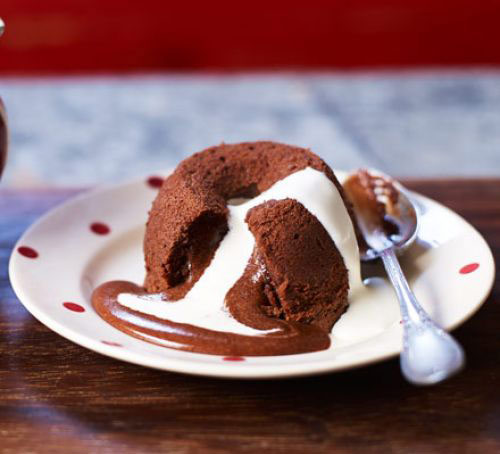
\includegraphics[width=0.7\textwidth]{Fotos/foto_sweet} \end{center}
% }
% \clearpage
\receitaemoji{Creme Brulé}{
\begin{itemize}
	\item 320g de creme de leite fresco
	\item Essência de baunilha
	\item 4 gemas
	\item 60g de açúcar fino
\end{itemize}
}{
\begin{enumerate}
	\item Esquentar o creme de leite junto com a baunilha
	\item Bater as gemas separadamente e acrescentar o açúcar
	\item Verter o creme quente sobre as gemas e ao mesmo tempo ir batendo
	      constantemente (temperagem) com um fouet. Evitar formar espuma
	      \begin{itemize}
		      \item É muito importante ir batendo, senão coagula e se perde a cremosidade.
	      \end{itemize}
	\item Verter os ramequins até preencher 2/3.
	\item Aquecer o forno a 150/180 $^\circ$C
	\item Colocar os ramequins numa forma e acrescentar água quente até no máximo
	      metade da altura dos ramequins.
	      \begin{itemize}
		      \item É basicamente um cozimento a banho maria no forno.
		      \item Se não tiver ramequins que suportam altas temperaturas, talvez dê para
		            utilizar xícaras ou potinhos de vidro.
	      \end{itemize}
	\item Levar ao forno por 30 a 40 minutos. Remover
	\item Esfriar na bancada. Depois, levar à geladeira sem cobrir, para não
	      formar uma película.
	\item Antes de servir, espalhar açúcar na superfície e passar o maçarico para
	      caramelizar.
\end{enumerate}
}

\receitatrescols{Overnight Oats}{

	\textsc{receita 1}\checkmark
	\begin{itemize}
		\item morango amassado
		\item açúcar ou maple ou mel
		\item 0,5 xícara de aveia
		\item 0,5 xícara de iogurte (grego)
		\item 0,5 limão espremido
		\item 0,5 xícara de leite
		\item Cobertura: morangos e framboesas
	\end{itemize}

	\textsc{receita 2}
	\begin{itemize}
		\item raspas de meia laranja
		\item açúcar ou maple ou mel
		\item amora preta amassada
		\item 15g de gengibre cristalizado
		\item 1 frasco de iogurte
		\item Cobertura: Amora preta
	\end{itemize}

	\textsc{receita 3}
	\begin{itemize}
		\item 10 g de chocolate em pó
		\item 20 g de aveia
		\item canela
		\item açúcar ou maple
		\item essência de baunilha
		\item 15 g de manteiga de amendoim
		\item 1 frasco de iogurte
		\item Cobertura: raspas de chocolate, framboesa e manteiga de amendoim
	\end{itemize}

}{

	\textsc{receita 4}
	\begin{itemize}
		\item 50 g de manga amassada
		\item 1 colher sopa de coco ralado
		\item 20 g de aveia
		\item essência de baunilha
		\item açúcar ou maple
		\item 1 frasco de iogurte
		\item Cobertura: manga em cubinhos e coco ralado
	\end{itemize}

	\textsc{receita 5}
	\begin{itemize}
		\item 1 cenoura ralada
		\item 20 g de aveia
		\item canela, noz moscada, baunilha
		\item maple ou açúcar
		\item 1 frasco de iogurte
		\item Cobertura: banana e nozes
	\end{itemize}

	\textsc{receita 6}
	\begin{itemize}
		\item 40 g de abacaxi picado
		\item 1 colher de sopa de coco ralado
		\item essência de baunilha
		\item 1 frasco de iogurte
		\item 1 colher de sopa de mel
		\item 20 g de aveia
	\end{itemize}
}{

	\textsc{receita 7}
	\begin{itemize}
		\item 10 g de chocolate em pó
		\item 1 colher de sopa de manteiga de amêndoas
		\item pitada de sal
		\item 1 frasco de iogurte
		\item 1 colher de sopa de mel
		\item 1 colher de sopa de coco ralado
		\item 20 g de aveia
	\end{itemize}

	\textsc{receita 8}
	\begin{itemize}
		\item 1 pote de iogurte
		\item Meia xícara de aveia
		\item Mel, aprox 20mL
		\item Chocolate meio amargo ralado
		\item Fruta congelada
	\end{itemize}

} {
	\begin{enumerate}
		\item Misturar tudo e guardar na geladeira no dia anterior.
		\item No dia seguinte colocar a cobertura.
	\end{enumerate} }
\receitaemoji{Crepe\label{rec:crepe}}{
		\begin{itemize}
			\item 1 ovo
			\item 2 colheres de chá de açúcar
			\item 1 pitada de sal
			\item 250 mL de leite integral
			\item 100g de farinha de trigo
			\item 20g de manteiga mole, derretida
			\item essência de baunilha, licor de laranja ou qualquer aromatizante de
			      preferência
		\end{itemize}
	}{
		\begin{enumerate}
			\item Juntar o ovo, açúcar, sal e bater com fouet. Mixer elétrico pode
			      desvirtuar a massa.
			\item Acrescentar 100mL de leite e misturar.
			\item Acrescentar a farinha de mexer bem até desfazer os grumos.
			\item Acrescentar aos poucos o restante do leite de misturar bem.
			\item Acrescentar a manteiga e misturar.
			\item Acrescentar o aromatizante.
			\item Deixar a massa repousar por pelo menos 1h antes de fritar. Ideal é
			      preparar com 5 horas de antecedência.
			\item Untar bem uma frigideira e aquecer em fogo médio/alto. Colocar uma
			      quantidade que preencha a frigideira bem finamente. Geralmente não precisa
			      untar a frigideira novamente.
			\item Colocar alguma cobertura se desejar. No caso do molho Suzette (receita
			      \ref{rec:molho_suzette}), se dobra o crepe em 4 e depois mergulha no molho,
			      ambos quentes, e é servido imediatamente.
		\end{enumerate}
	}

\receitaemoji{Molho Suzette para Crepe\label{rec:molho_suzette}}{
		\begin{itemize}
			\item 150 mL de suco de laranja
			\item 60 g de manteiga sem sal
			\item 40 g de açúcar
			\item 1 colher de sopa de licor de laranja
			\item raspas de laranja
		\end{itemize}
	}{
		\begin{enumerate}
			\item Derreter a manteiga em fogo médio e acrescentar o açúcar até
			      caramelizar.
			\item Acrescentar o suco de laranja, o licor e as raspas.
		\end{enumerate}
	}

\receitaemoji{Panqueca doce}{

		\textsc{30 panquecas}

		\begin{itemize}
			\item 3 ovos
			\item Meio litro de leite integral
			\item 40g de manteiga sem sal
			\item 40g de açúcar branco
			\item 2g de sal
			\item 225g de farinha de trigo
			\item rum, licor ou essência de baunilha ou aromatizante.
		\end{itemize}

		\textsc{10 panquecas}
		\begin{itemize}
			\item 1 ovo
			\item 0,3 xícara de leite
			\item 0,3 de xícara de creme de leite
			\item 1 colher de sopa de açúcar
			\item 0,75 xícara de farinha de trigo
			\item 1 pitada de sal
			\item 1 colher de sopa de manteiga derretida
			\item 0,5 colher de chá de essência de baunilha ou aromatizante.
		\end{itemize}
	}{
		\begin{enumerate}
			\item Peneirar a farinha junto com o sal e o açúcar
			\item Fazer um espaço no meio da farinha, acrescentar os ovos e ir misturando
			      com um fouet. Um misturador elétrico pode desvirtuar.
			\item Colocar o leite aos poucos para não formar pelotas, enquanto mistura
			\item Em panela separada, derreter a manteiga e juntar à massa, misturar.
			\item Acrescentar o aromatizante.
			\item Descansar a massa na geladeira por no mínimo 1h, idealmente 5.
			\item Untar uma frigideira e levar ao fogo médio/alto.
			\item Colocar uma quantidade de massa suficiente para cobrir o fundo da
			      frigideira, bem fino.
			\item Virar com uma espátula quando as bordas começarem a se soltar.
		\end{enumerate}
	}

\receitaemoji{Bolo de chocolate}{ % todo: adequar o texto.
		\textsc{Bolo de chocolate}
		\begin{itemize}
			\item 4 ovos
			\item 1 xícara (chá) de açúcar
			\item 1 xícara (chá) de chocolate em pó
			\item 1 xícara (chá) de óleo
			\item 1 xícara (chá) de água
			\item 2 xícaras (chá) de farinha de trigo
			\item 1 colher (sopa) de fermento
			\item Manteiga, farinha e chocolate para untar e polvilhar
		\end{itemize}
		\textsc{Calda de ganache}
		\begin{itemize}
			\item 200g de chocolate meio amargo
			\item 3/4 de xícara (chá) de creme de leite fresco
		\end{itemize}
	}{
		\begin{enumerate}
			\item Preaqueça o forno a 180ºC (temperatura média). Unte uma forma redonda ou
			      de pudim com manteiga, formando uma camada fina e uniforme.
			\item Faça uma misturinha meio a meio de chocolate em pó e farinha, e polvilhe
			      a forma toda. Desta maneira, o bolo não fica com aquela casquinha branca de
			      farinha. Reserve. Numa tigela, coloque a farinha, passando pela peneira.
			\item Na batedeira, ou numa tigela, coloque o açúcar e o chocolate em pó,
			      passando por uma peneira. Junte os ovos e o óleo. Na velocidade baixa (para
			      o chocolate não subir), bata os ingredientes, até que estejam bem
			      misturados.
			\item Aumente a velocidade e bata por mais alguns minutos. Caso prefira fazer
			      à mão, use um batedor de arame. Se estiver usando a batedeira, abaixe a
			      velocidade novamente e, aos poucos, vá adicionando a água e a farinha,
			      alternadamente, batendo apenas para misturar.
			\item Por último, adicione o fermento. Transfira a massa para a forma
			      preparada e leve ao forno preaquecido para assar por 30 minutos, até que o
			      palito saia limpo ao ser espetado no bolo.
			\item Retire do forno e deixe esfriar por 15 minutos. Coloque um prato de bolo
			      sobre a forma e, com o auxílio de um pano de prato vire de uma vez. Somente
			      quando o bolo estiver frio, espalhe a calda. Sirva a seguir.
		\end{enumerate}
	}

\receitaemoji{Mousse de chocolate}{
		\begin{itemize}
			\item 100 g de chocolate Cicao Mix (mistura de ao leite e meio-amargo)
			      \footnote{Essa quantia de chocolate foi dobrada. É possível que não precise
				      dobrar a quantidade caso use um chocolate mais duro.}
			\item 35 g de água
			\item Gelo
		\end{itemize}
	}{
		\begin{enumerate}
			\item Cortar o chocolate em pedaços grandes
			\item Misturar a água
			\item Levar ao microondas por 20 segundos.
			\item Mexer bem, levar por mais 20 segundos.
			\item Mexer, garantir que a mistura está bastante leve, sem grumos de
			      chocolate.
			\item Fazer um banho de gelo.
			\item  Colocar o chocolate no banho e bater bastante
			      com um mixer até ficar com uma consistência firme.
			\item Transferiro para um potinho
			\item Levar à geladeira por 1h para tomar consistência. Comer com moderação
		\end{enumerate}
	}

\receitaemoji{Mingau de aveia}{
		\begin{itemize}
			\item 200 mL de leite (ou 3/4 xícara de leite)
			\item 20 g de aveia   (ou 1/3 xícara de aveia)
			\item 1 punhado de cranberries
			\item (opcional) açúcar ou mel
			\item (opcional) gotas de chocolate
			\item (optional) amêndoas picadas para guarnecer
		\end{itemize}
	}{
		\begin{enumerate}
			\item Misturar tudo, colocar no fogo médio, mexendo sempre, até ficar espesso
			\item Colocar o guarnecimento, se desejar.
		\end{enumerate}
	}

\receitaemoji{Torta de Iogurte}{
	\begin{itemize}
		\item 4 ovos separados
		\item 70 g de açúcar
		\item 350 g de iogurte grego
		\item 40 g de maizena
		\item 4 g de fermento royal
		\item raspas de limão
		\item baunilha
	\end{itemize} }{
	\begin{enumerate}
		\item Bater as claras em neve e reservar. Demora menos do que parece, na mão! Em torno de 5 minutos.
		\item Bater as gemas com o açúcar até ficar bem claro e aumentar o volume.
		\item Acrescentar o iogurte, as raspas e a baunilha às gemas batidas e misturar bem
		\item Acrescentar a maizena junto com o fermento à mistura anterior até incorporar bem.
		\item Acrescentar as claras em neve aos poucos, com auxílio de uma espátula. Não usar batedeira. Usar
		      movimentos largos, para não remover o ar.\footnote{Caso não tenha espaço no recipiente da massa para
			      fazer essa transferência, transferir a clara em neve para um prato, e a massa para o recipiente da
			      clara, depois incorporar.}
		\item Untar uma forma de 22 cm de diâmetro com manteiga.
		\item Colocar em uma forma de 22 cm de diâmetro.
		\item Assar por 40-45 minutos a 170\grau{} C. A massa não fica muito dourada. Ela fica bem elástica assim
		      que sai do forno. Usar um palito para checar se está pronto.
		\item Depois deixar esfriar até temperatura ambiente sem a tampa. Pode consumir, mas fica melhor frio. A
		      massa afunda, é natural.
	\end{enumerate} }

\receitaemoji{Bolo de cenoura}{
	\begin{itemize}
		\item 3 cenouras grandes cortadas em rodelas
		\item 1 xícara de açúcar
		\item 0.5 xícara de óleo
		\item 3 ou 4 ovos
		\item 2 xícaras de farinha de trigo
		\item 1 colher de sopa de fermento
		\item 0.5 colher de chá de sal
		\item Manteiga para untar
	\end{itemize}
}{
	\begin{enumerate}
		\item Colocar as cenouras, açúcar, óleo e ovos no liquidificador, bater e
		      reservar
		\item Colocar a farinha de trigo, fermento, sal numa cuia, misturar bem,
		      adicionar os líquidos da etapa anterior, homogeneizar mas não bater muito.
		\item Untar a forma, colocar em forno pré-aquecido a 200\grau{} C por 40
		      minutos.
	\end{enumerate}
	\fotoreceita{0.7\textwidth}{./Fotos/bolo_cenoura.jpg}
}

\receitaemoji{Pão de mel em cubos}{
	\begin{itemize}
		\item 250 g de mel
		\item 200 g de açúcar
		\item 450 g de farinha de trigo
		\item 200 g de farinha  de amêndoas
		\item 100 g de nozes picadas
		\item 100 g de avelãs picadas
		\item 1/2 colher de chá de cardamomo moído
		\item 1/2 colher de chá de cravo em pó
		\item 1 colher de chá de canela em pó
		\item 100 g de frutas cristalizadas (p.e. cascas de laranja, de limão)
		\item 15 g de carbonato de amônio
		\item 4 colheres de sopa de rum1 ovo
		\item Manteiga e farinha para a assadeira
		\item Película de plástico para abrir a massa
		\item 3 colheres de sopa de geléia de damasco ou similar, 1 colher de sopa
		      de rum, 200 g de chocolate meio amargo para cobertura.
		\item 20 g de pistache picado, 50 g de cereja em calda, 50 g de amêndoas sem
		      pele, 50 g de nozes.
	\end{itemize}
}{
	\begin{enumerate}
		\item Numa panela levar o mel e açúcar em fogo baixo, misturando sempre, até
		      o açúcar se dissolver. Passar a massa para uma tigela e deixar esfriar.
		\item Pré-aquecer o forno a 175 \grau C.
		\item Untar uma assadeira com manteiga e passar um pouco de farinha
		\item Misturar a farinha e as amêndoas, avelãs, nozes, temperos e frutas
		      cristalizadas.
		\item Dissolver o carbonato de amônio com rum
		\item Adicionar um ovo à mistura de mel com açúcar e ir colocando aos poucos
		      a mistura de carbonato de amônio
		\item Amassar bem a massa e abri-la de modo uniforme entre as duas lâminas
		      de filme de plástico, na espessura da assadeira.
		\item Tirar a película de plástico e colocar a massa na assadeira. Assar por
		      20 minutos na grade do meio.\footnote{Feito para o nosso casamento!}
	\end{enumerate}
}



% \chapter{Informações adicionais}
\section{Tabelas}
\begin{table}[h]
	\centering
	\begin{tabular}[h]{c c}
		\hline
		Carne                  & Temperatura              \\
		\hline
		Vaca                   & 145 \grau F = 63 \grau C \\
		Porco                  & 145 \grau F = 63 \grau C \\
		Peixes e frutos do mar & 145 \grau F = 63 \grau C \\
		Carnes moídas          & 160 \grau F = 71 \grau C \\
		Ovos                   & 160 \grau F = 71 \grau C \\
		Frango                 & 165 \grau F = 74 \grau C \\
		Sobras                 & 165 \grau F = 74 \grau C \\
		\hline
	\end{tabular}
	\caption{Temperaturas mínimas do interior de carnes para checar se estão cozidas.
		Geralmente devem ficar por ao menos 3 minutos nessa temperatura}
	\label{tab:temperaturas_cozimento}
\end{table}

\begin{table}[h]
	\centering
	\begin{tabular}[h]{c c}
		\hline
		1 colher de chá  & $\approx$ 5 mL                    \\
		1 colher de sopa & $\approx$ 15 mL                   \\
		1 onça           & $\approx$ 28 g                    \\
		1 copo           & $\approx$ 240 mL                  \\
		1 kg             & $\approx$ 2.20 libra (lb)         \\
		1 libra (lb)     & 0.45 kg                           \\
		1 \emph{quart}   & 1.05 L                            \\
		\hline
		1 \grau C        & $\frac{5}{9} \left( F-32 \right)$ \\
		1 \grau F        & $\left(\frac{9}{5} C\right)+32$   \\
		\hline
		225 \grau F      & 105 \grau C                       \\
		250 \grau F      & 120 \grau C                       \\
		275 \grau F      & 135 \grau C                       \\
		300 \grau F      & 150 \grau C                       \\
		325 \grau F      & 165 \grau C                       \\
		350 \grau F      & 180 \grau C                       \\
		375 \grau F      & 190 \grau C                       \\
		400 \grau F      & 200 \grau C                       \\
		425 \grau F      & 220 \grau C                       \\
		450 \grau F      & 230 \grau C                       \\
		475 \grau F      & 245 \grau C                       \\
		\hline
	\end{tabular}
	\caption{Conversão de unidades}
	\label{tab:conversao_unidades}
\end{table}

\begin{table}[h]
	\centering
	\begin{tabular}[h]{c c}
		\hline
		tablespoon    & colher de sopa       \\
		teaspoon      & colher de chá        \\
		buttermilk    & leitelho             \\
		cup           & xícara               \\
		baking powder & fermento em pó       \\
		baking soda   & bicarbonato de sódio \\
		\hline
	\end{tabular}
	\caption{Traduções de frases comuns}
	\label{tab:traducoes_comuns}
\end{table}

% \rotatebox{90}{
\begin{landscape}
  \begin{table}[h]
    \centering
    \begin{tabular}[h]{c c c c c c}
      \hline
      Comida & Quantidade & Nível água & Tempo fervura & Tempo cozimento & Obs \\
      \hline
      Feijão & 2 tigelas & Metade & 16 min & $<$ 20 min & Deixar uns 10-15 min hidratando\\
      Beterraba & 4 betterabas grandes & Metade & $\sim$ 15 min & $\sim$ 12 min & - \\
      Acém & 900 g & Metade & - & $<$ 30 min & 30 min foi demais \\
      \hline
    \end{tabular}
    \caption{Tempos de cozimento na panela de pressão}
    \label{tab:tempos_cozimento_pp}
  \end{table}
\end{landscape}
% }
\clearpage

\section{Receitas rápidas}

\begin{itemize}
	\item Linguiça calabresa na frigideira fica boa por 5-10 minutos no fogo médio com tampa, virando
	      constantemente para não queimar. Se estiver bem tostada por fora mas fria por dentro, abaixar bem o fogo e
	      tampar. Checar a temperatura no interior com o termômetro.
	\item Para cozinhar beterrabas sem panela de pressão, cortar as mesmas pela metade, se estiverem muito
	      grandes, cobrir com água e ligar o fogo alto. Colocar um cronômetro a cada 30 minutos para alertar e ir
	      checar o nível da água e a textura, pois não pode tampar. No teste feito, 1h20 foi suficiente para
	      cozinhá-las ao ponto de poder passar uma faca por uma facilmente.
	\item Para cozinhar batata doce, colocar a batata cortada na água fria ainda. Demora cerca de 30 minutos
	      entre o tempo que a água começa a ferver e a batata estar cozida.
	\item Para cozinhar mandioca, cortar a mandioca para fazer caber, e não ter pedaços grandes demais.
	      Colocar na água e esquentar no máximo. Demora cerca de 1h para cozinhar. Depois, se quiser fritar no
	      airfryer, recobrir com óleo e sal e fritar a 200 \grau C por 10-14 minutos.
	\item Buttermilk, ou leitelho, é um derivado de leite ácido com pouca gordura. Para fazer um buttermilk
	      falso, pode-se utilizar leite e suco de limão/vinagre. Misturar e deixar por 10 minutos na bancada.
	\item Para fazer ghee, colocar a manteiga numa panela mais alta, e colocar o fogo o mais baixo possível. No
	      caso aqui, isso ainda é alto demais, então achar uma maneira de levantar a panela. Deixar evaporando por
	      um tempo, depois coar por um papel filtro. Tomar cuidado com o choque térmico da manteiga quente com o
	      vidro, para não estilhaçar.
	\item Para fazer grão de bico cozido, pernoitar na água, depois cozinhar com água, sal e louro por 40
	      minutos. O líquido que resta poderia, em teoria, ser batido para fazer algo similar a chantilly, mas
	      não é tão trivial. Eu testei, mas provavelmente precisaria de uma máquina, e ter colocado menos água.
\end{itemize}
\clearpage

\section{Informações, observações aleatórias}

\begin{itemize}
	\item Após utilizar feijão para fazer peso em alguma massa, não pode mais ser usado para cozinhar.
	\item Pimentão e cenoura, se ficarem fora de sacos na geladeira, ficam moles e enrugados. Cebola fica com
	      cheiro de geladeira e seca, esquisita, e a geladeira fica fedida. Alface fica super murcha, e tentar fazer
	      osmose deixando imersa em água não adianta muito.
\end{itemize}

\subsection*{Creme de leite e chantilly}
\begin{itemize}
	\item O creme de leite pode ter uma concentração de gordura na parte de cima. Então ele fica mais
	      consistente em cima do que em baixo. Um pouco de acidez é normal.
	\item O creme de leite está estragado quando fica amarelado
	\item Para fazer chantilly, o creme deve estar fresquíssimo
	\item O creme pode ser guardado na freezer por longos períodos. Tirar do frasco, homogeneizar, separar em
	      copos de $\pm$ 100 mL e guardar no freezer. Sempre deixar espaço para a expansão do gelo.
\end{itemize}

\subsection*{Bater clara em neve}
\begin{itemize}
	\item Para bater clara em neve sem equipamento, o processo parece mais penoso do que realmente é, se possuir
	      um Fouet. Colocar as claras numa tigela grande, e fazer movimentos com o braço e o punho também. Demorou
	      pouco da vez que eu fiz, 5 minutos, mais ou menos.
\end{itemize}




\subsection*{Tempos e métodos de requentamento}

\subsubsection*{Pizza de massa tradicional}
\begin{itemize}
	\item 160 \grau C por 8 minutos resultou numa pizza meio mole
	\item 200 \grau C por 10 minutos queimou um pouco, ficou pior que a 160 \grau C.
	\item 180 \grau C por 8 minutos parece que ficou bom
	\item No microondas ficou horrível.
\end{itemize}

\subsubsection*{Pan pizza}
\begin{itemize}
	\item De forma geral, 180 \grau C por 10 minutos serve. Microondas fica pior, mas comível.
	\item As pizzas do Pizza Hut e Domino's requentam melhor que as pizzas tradicionais.
\end{itemize}

\subsubsection*{Esfiha fechada}
\begin{itemize}
	\item 180 \grau C por 5-8 minutos ficou bom.
\end{itemize}

%%% Local Variables:
%%% mode: latex
%%% TeX-master: "main"
%%% End:

\end{document}

%%% Local Variables:
%%% mode: latex
%%% TeX-master: t
%%% End:
